\documentclass[oneside,senior,etd]{BYUPhys}

\usepackage[utf8]{inputenc}
\usepackage[russian]{babel}
\usepackage{tikz}
\usepackage{ntheorem}
\usepackage{tabu}
\usepackage{mathtools}
\usepackage{graphicx}
\usepackage{fixltx2e}
\usepackage{caption}
\usepackage{float}
\usepackage{graphicx}
\usepackage{subcaption}
\usepackage{amssymb}
\usepackage{tabularx} % extra features for tabular environment
\usepackage{amsmath}  % improve math presentation
\usepackage{graphicx} % takes care of graphic including machinery
\usepackage[margin=1in,letterpaper]{geometry} % decreases margins
\usepackage{cite} % takes care of citations
\usepackage[final]{hyperref} % adds hyper links inside the generated pdf file


\usetikzlibrary{shapes.geometric,shapes.symbols,positioning,decorations.pathmorphing}

\DeclareMathOperator*{\argmax}{argmax} % thin space, limits underneath in displays
\DeclareMathOperator*{\argmin}{argmin} % thin space, limits underneath in displays
\DeclareMathOperator*{\Motimes}{\text{\raisebox{0.25ex}{\scalebox{0.8}{$\bigotimes$}}}}


\newcommand*\circled[1]{\tikz[baseline=(char.base)]{
            \node[shape=circle,draw,inner sep=2pt] (char) {#1};}}
   
\hypersetup{
    linktocpage=true,           % ссылки с номера страницы в оглавлении, списке таблиц и списке рисунков
    plainpages=false,           % Forces page anchors to be named by the Arabic form  of the page number, rather than the formatted form
    colorlinks,                 % ссылки отображаются раскрашенным текстом, а не раскрашенным прямоугольником, вокруг текста
    linkcolor=blue,      % цвет ссылок типа ref, eqref и подобных
    citecolor=blue,      % цвет ссылок-цитат
    urlcolor=blue,        % цвет гиперссылок
    pdflang={ru}
}
\graphicspath{{./images/}}
\fixmargins
\oneandhalfspace

\DeclareMathOperator*{\argmax}{argmax} % thin space, limits underneath in displays
\DeclareMathOperator*{\argmin}{argmin} % thin space, limits underneath in displays
\DeclareMathOperator*{\Motimes}{\text{\raisebox{0.25ex}{\scalebox{0.8}{$\bigotimes$}}}}

\newcommand\myeq{\mathrel{\overset{\makebox[0pt]{\mbox{\normalfont\tiny\sffamily def}}}{=}}}

\Chair{Кафедра Исследования Операций}
\Lab{~}
\Year{2019}
  \Month{Июнь}
  \City{Москва}
  \AuthorText{Автор}
  \Author{Кононов Сергей Владиславович}
  \AuthorEng{Kononov Sergey}
  \AcadGroup{411}

  \TitleTop{Исследование модельной игры преподавателя и студента}
  \TitleBottom{с применением свёртки Гермейера у студента} % leave empty if you don't need it
  \TitleTopEng{Research into teacher-student model game with use of}
  \TitleBottomEng{Germeyer's scalarization for student} % leave empty if you don't need it  
  \docname{Выпускная квалификаионная работа}
  \Advisor{Поспелова Ирина Игоревна}
  \AdvisorDegree{к.ф.-м.н\\}

\Abstract{
В работе проводится исследование в области применения 
сверток в игре с векторной функцией выигрыша. Анализируются оптимальные стратегии и значения игры при различных степенях дискретизации непрерывной 
модельной игры преподавателя и студента. 
}
\AbstractEng{Abstract}


%%%% DON'T change this. It is here because .sty does not support cyrillic cp properly %%%%
\University{Московский Государственный Университет имени М.В.Ломоносова}
\Faculty{Факультет Вычислительной Математики и Кибернетики}
\GrText{группа}
\AdvisorText{Научный руководитель}
\AbstractText{Аннотация}


\begin{document}

	\makepreliminarypages % Титульная страница

	\tableofcontents % Оглавление
	
	\section{Введение}

\qquad Теорией игр называется математическая теория принятия решений
в конфликтных ситуациях. В простейших моделях рассматривается \textit{лицо
принимающее решение} (ЛПР), которое выбирает своё действие из некоторого
множества стратегий. Считается, что задана \textit{целевая функция},
которая отражает интересы ЛПР и зависит от выбранной им стратегий.
Задача принятия решений состоит в том, чтобы найти стратегию, 
при которой достигается максимум целевой функции. Отличие конфликтной ситуации
заключается в том, что решения принимаются не одним лицом, 
а всеми участниками конфликтной ситуации и функция выигрыша
каждого индивида зависит не только от его решения, но 
и от решения остальных участников.  Модель такого вида называется --
игрой, а участники конфликта -- игроками. В рамках данной работы
будет рассмотрена задача из теории \textit{некооперативных игр} -- 
игр, в которых игроки действуют самостоятельно, независимо друг 
от друга. Определим формально модель игры с несколькими участниками в общем виде.

Есть конечное \textit{множество игроков} $A = \{1, 2, ..., m \}$. 
Каждый игрок $a \in A$ имеет 
\textit{множество чистых стратегий} $S_a=\{1,2,...,n_a\}$, при этом 
\textit{игровой ситуацией} или просто \textit{ситуацией}
называется $m$-мерный вектор:
\begin{equation}
	\label{eq:game_situation}
	\textbf{s} = (s_1, \, s_2, \ldots , \, s_m) \in
	S_1 \times S_2 \times \ldots \times S_m,
\end{equation}
где $X \times Y$ обозначает декартово произведение множеств $X$ и $Y$.
\textit{Функция выигрыша} $F_a, \: a \in A$ обозначает выигрыш игрока при
конкретной ситуации в игре. Она определена для каждого игрока и имеет 
вид:
\begin{equation}
	\label{eq:single_dim_payoff_function}
	F_a: S_1 \times S_2 \times \ldots \times S_m \rightarrow 
	\mathbb R, \; a \in A
\end{equation}

\newtheorem{Defenition}{Определение}
\begin{Defenition}
	Игрой в нормальной форме называется совокупность:
	\begin{equation}
		G = \big \langle A, S, F \big \rangle
		\label{eq:normal_form_game}
	\end{equation}
	где: 
 
	$ A = \{1, \, 2, ..., \, m\}$ - множество игроков,

	$ S = \{S_1, \, S_2, ..., \, S_m\}$ - множество наборов чистых
	стратегий игроков,

	$ F = \{F_1, \, F_2, ..., \, F_m\}$ - множество функций выигрыша
	игроков. 
	\cite{vasin}
\end{Defenition}

\begin{flushleft}
Теперь введём фундаментальное понятие в теории игр --
\textit{равновесие по Нэшу}:
\end{flushleft}
\begin{Defenition}
	Ситуация $\textbf{s} = (s_1^0, \, s_2^0, ..., \, s_m^0)$ называется
	\cite{vasin} равновесием по Нэшу в игре \eqref{eq:normal_form_game},
	если:
	\begin{equation}
		\max \limits_{s_a \in S_a} 
		F_a(s_1^0, ..., s_{a-1}^0, s_a, s_{a+1}^0..., s_m^0)=
		F_a(s_1^0, ..., s_{a-1}^0, s_a^0, s_{a+1}^0..., s_m^0),
		\: \forall \; a \in A.
		\label{eq:nash_equilibrium}
	\end{equation}
\end{Defenition}

Смысл этого определения заключается в том, что 
при ситуации в игре, которая является равновесием по Нэшу,
ни одному игроку индивидуально не выгодно отклоняться от своей текущей 
стратегии.

До этого мы рассматривали функции выигрыша 
игроков, которые имели вид
\eqref{eq:single_dim_payoff_function}, т.е. каждому игроку 
соответствовало одно значение, зависящее от ситуации игры.
Однако, не всегда интересы могут быть выражены одним критерием. Часто 
возникают разные оценки качества принимаемого решения, причем они могут 
быть противоречивыми и их нельзя свести друг у другу. Например 
характеристиками решения могут быть такие значения 
как \textit{(время, деньги)} или 
\textit{(математическое ожидание, дисперсия)}. Следуя этим рассуждениям  
рассмотрим такое обобщение игры \eqref{eq:normal_form_game}, что функция
выигрыша игроков имеет вид:
\begin{equation}
	F: S_1 \times S_2 \times ... \times S_m \rightarrow \mathbb R^n
	, \; n \in \mathbb{N}
	\label{eq:multidem_payoff_function}
\end{equation}

Такое обобщение ближе к реальным ситуациям
в которых критерием выбора представляет собой несколько значимых параметров.
Для примера такой игры можно привести задачу выбора машины: 
допустим покупателю важно чтобы машина имела большую мощность, 
достаточный уровень безопасности 
и мало стоила, продавцу же важно, чтобы она стоила как можно дороже и 
кроме того следует продавать те машины, которые плохо покупают. 
Таким образом мы получили игру, в которой игроки имеют три и два критерия
соответственно, которые важны для них при выборе стратегии. 
Пока что мы допустили существование игры с функцией выигрыша
вида \eqref{eq:multidem_payoff_function}. Формализация и подробное 
описание будет позже.

Приведённые выше обобщения приводят нас к другому разделу
математики, а именно -- \textit{многокритериальной оптимизации}.
Рассмотрим следующую задачу которая относится к этой области.
\begin{equation}
	\label{eq:multi_criteral_problem}
	\Max \limits_{x \in X} F(x), \; F(x)=({f}_1(x),\ldots, {f}_m(x))
	, \; X \subseteq \mathbb{R}^n,
\end{equation}
где $f_i: \mathbb{R}^n \rightarrow \mathbb{R}, \; i = 1, \ldots, m.$
Это задача заключается в том, что у нас есть $n$-мерная функция,
которая представляет собой множество значений критериев, зависящих
от параметров, которые принадлежат некоторому множеству.
Особенность заключается в том, что правило сравнения двух векторов
не определено однозначно, т.е. в общей задаче не всегда можно точно сказать,
какой из двух векторов значений функции предпочтительнее.
В примере про покупку автомобиля можно сказать, что если 
одна машина более мощная и менее дорогая чем вторая, то она предпочтительнее,
однако, если она более мощная, но при этом и стоит дороже, то
правило их сравнения не определено. 
Введём понятие \textit{оптимальных (эффективных) по Парето} и 
\textit{оптимальных (эффективных) по Слейтеру}
векторов в задаче \eqref{eq:multi_criteral_problem}.
И значением максимума в задаче \eqref{eq:multi_criteral_problem},
который в отличие от скалярного максимума записывается с заглавной буквы,
будем считать \textit{множество Слейтера} в критериальном пространстве 
$\mathbb{R}^m$.

\begin{Defenition}
	Допустимое решение $\hat{x}\in{X}$ называется 
	оптимальным по Слейтеру (оптимальным по Парето) для задачи		
	\eqref{eq:multi_criteral_problem},
	если \textbf{не} существует $x\in{X}$ такого, что 
	$f_k(x)>f_k(\hat{x}) \; (f_k(x) \geqslant f_k(\hat{x}))$ для всех
	$k = 1, \ldots ,m$. Множество всех оптимальных по Слейтеру 
	(оптимальных по Парето) решений задачи 
	\eqref{eq:multi_criteral_problem} называется 
	\textit{множеством Слейтера} (\textit{множеством Парето}) 
	задачи \eqref{eq:multi_criteral_problem}.
	\cite{ehrgott}
\end{Defenition}

Другими словами это такое множество значений, 
при котором значение каждого частного показателя, характеризующего систему, 
не может быть улучшено без ухудшения других.

Для поиска множества Слейтера существуют разные методы
\cite{ehrgott}, \cite{blackwell},
в текущей работе исследуется \textit{метод свёрток} \cite{germeyer}. 
Метод заключается в том, что задача \eqref{eq:multi_criteral_problem}
заменяется параметрическим семейством скалярных задач:
$$
	\max\limits_{x \in X} C(\{f_i\}_{i=1}^{m}, \lambda, x), \;
	\lambda \in \Lambda
$$
где: 
 
$C$ – функция свертки частных критериев $\{f_i\}_{i=1}^m$ задачи 
\eqref{eq:multi_criteral_problem} в единый скалярный критерий,
 
$\lambda$ – параметр свертки заданный на некоторой
области определения $\Lambda$.
\newline

В текущей работе рассмотрены две различные свёртки --
\textit{линейная свёртка} и \textit{обратная логическая свёртка}:

\begin{Defenition}
	Линейной свёрткой с параметром $\lambda$ для функции критериев задачи
	\eqref{eq:multi_criteral_problem} называется 	\cite{ehrgott}
	функция:
	\begin{equation}
		\label{eq:linear_scalarization}
		L(\{f_i\}_{i=1}^{m}, \lambda, x) = 
		\sum_{i=1}^{n} \lambda_i f_i,
	\end{equation}
	где  
	\begin{equation}
		\label{eq:Lambda}
		\lambda \in 
		\Lambda = \{
			(\lambda_1, \ldots, \lambda_m) \:
			| \: \sum_{i=1}^m \lambda_i = 1, \: 
			  \lambda_i \geq 0 \; i = 1, \ldots m 
		\}.		
	\end{equation}
\end{Defenition}

\begin{Defenition}
	Свёрткой Гермейера с параметром $\mu$ для 
	функции критериев задачи \eqref{eq:multi_criteral_problem}
	называется \cite{germeyer} функция:
	\begin{equation}
		\label{eq:germeyer_scalarization}	
		G(\{f_i\}_{i=1}^{m}, \mu, x)=
		\min \limits_{i: \mu_i > 0} \mu_i f_i,
	\end{equation}
	где 
	\begin{equation}
		\label{eq:Mu}	
		\mu \in 
		M = \{
			(\mu_1, \ldots, \mu_m) \:
			| \: \sum_{i=1}^m \mu_i = 1, \: 
			  \mu_i \geq 0 \; i = 1, \ldots m 
		\}.
	\end{equation}
\end{Defenition}

Применение линейной свёртки в задачах вида
\eqref{eq:multi_criteral_problem} обосновывается теоремой Карлина:

\newtheorem{Theorem}{Теорема}
\begin{Theorem}[Карлин]
	Рассмотрим задачу \eqref{eq:multi_criteral_problem}. 
	Пусть множество $X \subseteq \mathbb{R}^n$ выпукло,
	а функции $f_1, \ldots, f_m$ - вогнуты на нём.
	Если $x^*$ – эффективная по Парето точка,
    тогда существует вектор $\lambda \in \Lambda$ из 
    \eqref{eq:Lambda} такой, что $x^*$ является точкой 
    максимума функции \eqref{eq:linear_scalarization} по переменной
    $x$. \cite{carlin}
\end{Theorem}

Гермейером была предложена свертка, которая также аппроксимирует 
множество Слейтера. Её применение в многокритериальных 
задачах обосновывается следующей теоремой Гермейера:

\begin{Theorem}[Гермейер]
	Рассмотрим задачу \eqref{eq:multi_criteral_problem}.     
    Пусть $x^*$ - эффективная по Слейтеру точка, 
    причем $f_1(x^*)>0, \ldots, f_m(x^*)>0$.
    Тогда существует вектор $\mu \in M$ из \eqref{eq:Mu} 
    и $x^*$ является точкой максимума функции 
    \eqref{eq:germeyer_scalarization} по переменной $x$. 
    \cite{germeyer} 
\end{Theorem}

В работе будет использоваться модификация свёртки Гермейера -
\textit{обратная логическая свертка}. Она отличается
только тем, что веса (параметры свёртки) стоят в знаменателе, 
а не в числителе.

\begin{Defenition}
	Обратной логической свёрткой с параметром $\mu$ для 
	функции критериев задачи \eqref{eq:multi_criteral_problem}
	называется функция:
	
	\begin{equation}
		G(\{f_i\}_{i=1}^{m}, \mu, x)=
		\min \limits_{i: \mu_i > 0} \frac{f_i}{\mu_i},
		\label{eq:RL_scalarization}	
	\end{equation}
	где $\mu \in M$ определено в \eqref{eq:Mu}.
\end{Defenition}

Вернёмся к рассмотрению некооперативных игр.
Если множество чистых стратегий у игроков конечно, то игра
называется \textit{конечная}. Для конечной игры
определим обобщение модели, 
а именно - \textit{смешанное расширение игры}.
Смысл смешанного расширения игры заключается в том, что
каждый игрок выбирает любую из своих чистых стратегий с некоторой
фиксированной вероятностью, и его стратегией является
не одна чистая стратегия, а вероятностное  распределение над множеством 
его чистых стратегий. Выигрышем игрока в таком случае считаем взвешенный
выигрыш по всем ситуациям с весами соответствующими вероятностям данной
ситуации. Определим эти понятия формально.

Пусть в игре 
$G = \big \langle A, S, F \big \rangle$. $A$ -- конечное множество игроков,
$A = \{1, 2, ..., m\}$, причём
множества чистых стратегии $S_a=\{1, 2,...,n_a\} \; a \in A$ конечны.  
\textit{Смешанной стратегией} игрока $a \in A$ называется 
вероятностное распределение над множеством чистых стратегий 
$S_a$ игрока $a \in A$:
$$
	\pi^a \in P_a
	= \{ 
		(\pi^a_1, \pi^a_2, ..., \pi^a_{n_a}) \in [0,1]^{n_a}\: | \:
		\sum \limits_{i=1}^{n_a} \pi^a_i = 1
	\}
$$
где $\pi^a_i$ - это вероятность выбора игроком $a \in A$ чистой 
стратегии $s^a_i$ в качестве реальной стратегии игрока,
а $[0,1]^n$ обозначает $n$-ую декартову степень отрезка $[0,1]$.
Симплекс $P_a$ называется \textit{множеством смешанных стратегий игрока}.
Введём обозначение для заданного набора стратегий:
$$
	\pi = (\pi^1, \ldots, \pi^m) \in P = P_1 \times \ldots \times P_m,
$$
и вероятности реализации ситуации \textbf{s} из 
\eqref{eq:game_situation}:
$$
	p(s|\pi) = \prod_{a \in A} \pi^a_{s_a}.
$$
Тогда математическое ожидание выигрыша игрока $a \in A$
задаётся функцией: 
$$
	\overline F_a(\pi) = \sum \limits_{s \in S}p(s|\pi)F_a(s),
$$
где функция $F_a$ - определена в \eqref{eq:normal_form_game}.
Таким образом смешанное расширение игры в нормальной форме определяется
следующим образом:

\begin{Defenition}
	Смешанным расширением игры в нормальной форме называется 
	совокупность:
	\begin{equation}
		\overline G = \lbrace A, P, \overline F \rbrace	
		\label{eq:ext_normal_form_game}
	\end{equation}
	где: 
 
	$A = \{1, 2, ..., m\}$ -- множество игроков,

	$P = P_1 \times \ldots \times P_m$ -- множество наборов смешанных 
	стратегий игроков,

	$\overline F = \{
		\overline F_1, \overline F_2, ..., \overline F_m
	\}$
	-- множество функций выигрыша игроков.
\end{Defenition}

Ситуации равновесия \eqref{eq:nash_equilibrium} игры $\overline G$
будем называть \textit{ситуациями равновесия в смешанных стратегиях игры $G$}
или \textit{смешанными равновесиями по Нэшу}. 

Теперь в игре \eqref{eq:ext_normal_form_game} будем считать, что функции
выигрыша $F_a, \; a \in A$ имеют вид \eqref{eq:multidem_payoff_function}.
Обозначим через $S_a(\pi || a), \; a \in A$ множество Слейтера задачи  
$
	\Max \limits_{\pi \: : \: \pi^a \in P^a} \overline F_a(\pi), 
$
в которой все координаты $\pi$, кроме $a$ фиксированы.

\begin{Defenition}
	Решением игры \eqref{eq:ext_normal_form_game} согласно \cite{blackwell} 
	является множество ситуаций $P^*$:
	\begin{equation}
		P^* = \{ 
			\pi = (\pi^1, \ldots, \pi^m) \in P \: | \:
			\pi^a \in S_a(\pi || a), \; a \in A
		\}
		\label{eq:game_solution}
	\end{equation}
\end{Defenition}

В случае конечных многокритериальных игр Шепли свел \cite{shapley}
описание данного множества к семейству задач поиска значений 
скалярных игр с 
функциями выигрышей -- ЛС частных критериев при произвольном наборе
весовых коэффициентов, своих у каждого игрока.
В случае скалярной игры осреднение однозначно, а  для скаляризованной
вектор-функции могут быть разные варианты.

Целью данной выпускной квалификационной работы является исследование 
применения разных сверток в игре с векторным выигрышем. % Введение
	\section{Постановка задачи}

Рассматриваются два игрока -- Студент, далее обозначается \textbf{С},
и Преподаватель, далее обозначается \textbf{П}, которые имеют противоположные интересы.
Критерий интересов составляют две велечины, первая из которых является эффективностью
работы \textbf{С} в научной сфере, а второй его эффективностью на подработке.

\textbf{С} выбирает долю $x$ рабочего времени, которую он тратит на подготовку
диплома, оставшееся рабочее время $1-x$ он тратит на подработку. Считается, что производительность \textbf{С} при любых занятий падает с увеличением 
отводимого на них времени, эффективность труда \textbf{С} зададим функцией $\sqrt{x}$
и $\sqrt{1-x}$ соответственно. \textbf{С} может распределять свое время между двумя 
видами деятельности, т.е. имеет множетсво стратегий $x\in X = \{0, 1\}$, 
причём он может использовать смешанные стратегии.

\textbf{П} выбирает -- отностится к \textbf{С} требовательно, способствую 
написанию диплома и мешая подработке или же не обращать на него внимания не 
мешая подработке и не помогая с дипломом. \textbf{П} имеет множество стратегий 
$y \in Y=\{1, 2\}$, причём тоже может использовать смешаные стратегии.

Получаем следующую вектор-функция выигрыша:
\begin{equation}
	F(x, y)=
	\big(f_1(x,y), f_2(x,y)\big) =
	\Big(
		\frac{y\sqrt{x}}2,
		\frac{\sqrt{1-x}}y
	\Big)
	\label{eq:player_criterion}
\end{equation}

\textbf{П} стремится минимизировать (выборая $y \in Y = \{1,2\}$)
вектор-функцию выигрыша $F(x, y)$, а игрок \textbf{С} - максимизировать
 (выбирая $x \in X=[0,1]$).

Мы будем рассматривать конечную игру \textbf{C --- П}, полученную из исходной дисеретизацией множества $X$ конечным множеством точек:
$$
	X^T = \{
		0, \; 
		\frac{1}{T}, \; 
		\frac{2}{T}, \; 
		\ldots, \; 
		\frac{T-1}{T}, \;
		1
	\}, \;\; T \in \mathbb{N}
$$

Теперь задачу можно представить в виде многокритериальной игры двух лиц 
с противоположными интересами:


\begin{equation}
	G = \big \langle A, P, \textbf{F} \big \rangle
\end{equation}
	где: 
 
	$ A = $\{\textbf{C}, \textbf{П}\} - множество игроков,

	$ P = \{X^T, \, Y\}$ - множество наборов чистых
	стратегий игроков,
	
	$ \textbf{F} = \{F, \, -F\}$ - множество вектор-функций выигрыша
	игроков.
\newline
Игра записана в чистых старатегиях. Мы же допустим, что игроки будут 
использовать смешанные стратегии. 
В работе исследуются случаи дискретизации, когда $T=1$ и тогда 
множество $X^1=\{0, 1\}$, и когда 
$T=2$, тогда множество чистых стратегий \textbf{С}
примнимет вид $X^2=\{0, \frac{1}{2} ,1\}$.
В каждом случае необходимо решить игру, т.е. найти
равновесия Нэша в смешанных стратениях. Составим план, по которому
будет проходить поиск решений \eqref{eq:ext_normal_form_game}.

\hspace{3mm}

\textbf{(1)} 
Игроки используют смешанные стратегии, поэтому стратегий \textbf{С} и
\textbf{П} будет распределение вероятностей $p \in P$ и 
$q \in Q$ над множествами $X^T$ и $Y$
соответсвенно. Где $P$ и $Q$ -- все допустимые
распределения над этими множествами.
Следовательно заменим вектор-функцию выигрыша каждого
игрока на матожидание этой функции по распределению вероятностей его
стартегии. Для \textbf{С} и \textbf{П} функции принимают вид 
$\mathbb{E}_x [F(x,y)]$ и $\mathbb{E}_y [-F(x,y)]$.

\hspace{3mm}

\textbf{(2)}
Каждый игрок выбирает функцию свёртки, которая будет аппроксимировать его
множество слейтера $S_a$. В данной работе исследуется случай, когда
игрок \textbf{С} выбирет \textit{обратную логическую свёртку}, 
а игрок \textbf{П} \textit{линейную свёртку}. После чего игроки 
применяют свёртку к осреднённой вектор-функции выигрыша.
Для \textbf{С} и \textbf{П} функции принимают вид 
$G(\mathbb{E}_x [F(x,y)], p, y)$ и $L(\mathbb{E}_y [-F(x,y)], x, q)$.

\hspace{3mm}

\textbf{(3)}
Далее игроки получают скалярный критерий, который зависит от 
чистых стратегий противника. Поскольку игроки используют смешанные стратегии,
то на 3 -- ем этапе игроки осредняют скаляризованные критерии по 
стратегиям противника. Мы получили функции выигрыша игроков, которые
зависят от их смешнных стратегий.
Для \textbf{С} и \textbf{П} функции принимают вид 
$$
	\overline G(p, q, \mu) =
	\mathbb{E}_y [G(\mathbb{E}_x [F(x,y)], p, y, \mu)]
$$ и $$
	\overline L(p, q, \lambda) = 
	\mathbb{E}_x [L(\mathbb{E}_y [-F(x,y)], x, q, \lambda)].
$$

\textbf{(4)}
Теперь мы получили игру в смешанных стратегиях и нам необходимо решить игру
т.е. найти все возможные равновесия Нэша \eqref{eq:nash_equilibrium}
при фиксированных параметрах свёртки. 
Стратегии, которые являются решениями будем называть 
\textit{оптимальными стратегиями}. В конкретном случае они определяются
следующим образом:

\begin{Def}	
	Пара стратегий $(p^0, q^0) \in P \times Q$
	называется оптимальными, если для некоторых 
	$\lambda$, $\mu$ верно:
	\begin{equation}
		\begin{cases} 
			p^0(q^0, \lambda) = 
			\arg \min \limits_{p \in P} \overline L(p, q^0, \lambda) \\ 
			q^0(p^0, \mu) = 
			\arg \min \limits_{q \in Q} \overline G(p^0, q, \mu) \\
		\end{cases}
	\label{def:optimal_strategy}
	\end{equation}
	Использованы следующие обозначения:
	\begin{gather*}
		\arg \max \limits_{x \in X} f(x) = 
		\{ x^* \in X \: | \: f(x^*) = \max \limits_{x \in X} f(x)\}
		\\
		\arg \min \limits_{x \in X} f(x) = 
		\{ x^* \in X \: | \: f(x^*) = \min \limits_{x \in X} f(x)\}
	\end{gather*}
	Множесво всех оптимальных пар обозначим через $\mathbb{O}_T$,
	где $T$ -- означает степень дискретизации для конкретной задачи.
\end{Def}
%Рассмотрим случай, когда \textbf{С} использует обратную логическую свертку,
%с парамером $\mu$, a \textbf{П} использует линейную
%свертку с параметром $\lambda$. Тогда множество оптимальных решений
%принимает следующий вид:

%\begin{gather*}
%	\begin{cases}
%		x^*=\arg \max \limits_{x \in X}
%			G(\{f_1, f_2\}, \mu, x, y^*) \\
%		y^*=\arg \min \limits_{y}   
%			L(\{f_1, f_2\}, \lambda, x^*, y)
%	\end{cases}
%\end{gather*}

%Поскольку игроки используют смешанные стратегии т.е. распределения %вероятностей
%$\rho_x(x)$ и $\rho_y(y)$ над чистыми стратегиями $x \in X$ и $y \in Y$. 
%Далее каждый игрок осредняет свою функцию выигрыша по стратегиям противника

%$$ \overline G(\{f_1, f_2\}, \mu, q, p) = 
%\iint \limits_{PQ} G(\{f_1, f_2\}, \mu, q, p) \rho_x(x) \rho_y(y)dxdy$$
%$$ \overline L(\{f_1, f_2\}, \lambda, q, p) = 
%\iint \limits_{PQ} L(\{f_1, f_2\}, \lambda, q, p) \rho_x(x) \rho_y(y)dxdy$ % Постановка задачи
	\section{Постановка задачи (Парметр дискретизации Т=1)}

Сначала рассмотри случай с параметром $T=1$. Тогда множество $X^1=\{0, 1\}$.
Игроки используют смешанные стратегии т.е. распределение над своими чистыми 
стратегиями.
Чистыми стратегиями игроков \textbf{С} и \textbf{П} являются $X^1=\{0, 1\}$ и 
$Y=\{1,2\}$ соответсвенно. Эти множества дискретны и равномощны, поэтому 
распределения задаются в виде векторов: 
$$
	(p_1, p_2) \in P_2 = \{
		(p_1, p_2) \in \mathbb{R}_+^2 \; | \; p_1 + p_2 = 1)
	\},
$$
где $
	\mathbb{R}_+^n = \{ x \in \mathbb{R}^n \: | \: 
	x_i \geqslant 0 \; i = 1, \ldots n\}
$.
Множество $Q_2=P_2$, введено для наглядности. 
Смешанные стратеги игроков \textbf{С} и \textbf{П} будем обозначать
$q=(q_0,q_1) \in Q_2$ и $p=(p_0,p_1) \in P_2$ соответсвенно, причём:
\begin{equation}
	\begin{tabu} to 0.9 \textwidth {X[c] X[c]}
		$P(X=0)=q_0$ & $P(Y=1)=p_0$ \\
		$P(X=1)=q_1$ & $P(Y=2)=p_1$ \\
	\end{tabu}	
	\label{eq:probability_1}
\end{equation}

Введём обозначения $q := q_1$ и $p := p_1$, тогда $q_0 = 1-q$ и $p_0 = 1 - p$. 
Игрок \textbf{С} использует смешаную стратегию  $(q_0,q_1)$, тогда
его векторный критерий \eqref{eq:player_criterion} приобретает вид: 
$$
	F_\textrm{C}(q,y)=
	\big \langle
		q_0\frac{y\sqrt{0}}{2} + 
		q_1\frac{y\sqrt{1}}{2};
		q_0\frac{\sqrt{1}}{y} +
		q_1\frac{\sqrt{0}}{y}
	\big \rangle 
	= 	
	\big \langle
		\frac{q_1y}{2};
		\frac{q_0}{y}
	\big \rangle 
$$
Игрок \textbf{П} использует смешаную стратегию  $(p_0,p_1)$, тогда
его векторный критерий \eqref{eq:player_criterion} приобретает вид: 
\begin{gather*}
	F_\textrm{П}(x,p)=
	\big \langle 
		(1-p)\frac{1 \cdot \sqrt{x}}{2} + p \frac{2 \cdot \sqrt{x}}{2}; \;
		(1-p)\frac{\sqrt{1-x}}{1}+p\frac{\sqrt{1-x}}{2} 
	\big \rangle=
	\\
	=\frac{1}{2}
	\big \langle
		(p+1)\sqrt{x}; \;
		(2-p)\sqrt{1-x}
	\big \rangle
\end{gather*}

Далее игрок \textbf{С} использует \textit{обратную логическую свёртку}
\eqref{eq:germeyer_scalarization}:
$$
	G(y, q, \mu) = 
	\min \limits_{i: \mu_i > 0} \{\frac{q_1y}{2\mu_0};\frac{q_0}{y\mu_1}\},
$$
a игрок \textbf{П} использует \textit{линейную свёртку}
\eqref{eq:linear_scalarization}:
$$
	L(p, x, \lambda) = 
	\lambda_0 (p+1)\sqrt{x} + \lambda_1 (2-p)\sqrt{1-x}.
$$

После чего игрок \textbf{С} осредняет свёртку критерия по стратегиям игрока \textbf{П},
т.е. по переменной $y$:
$$
	\overline G(p,q,\mu)=
	p\min{\{\frac{q}{\mu};
	\frac{1-q}{2(1-\mu)}\}}
	+(1-p)\min\{\frac{q}{2\mu};\frac{1-q}{1-\mu}\},
$$
а игрок \textbf{П} осредняет свёртку критерия по стратегиям игрока \textbf{С},
т.е. по переменной $x$:
$$
	\overline L(p, q, \lambda) =
	\frac{1}{2}\big \{q(3\lambda+p-2)+(2-p)(1-\lambda)\big \}.
$$

Мы определили функции выигрыша игроков. Теперь задачу можно формализовать и представить как семейство игр двух игроков в нормальный форме:

$$
	\bigg \langle 
		\{\textrm{\textbf{С}, \textbf{П}}\},		
		\{Q, \: P\},		
		\{\overline G(p,q,\mu), - \overline L(p,q,\lambda) \}
	\bigg \rangle 
	, \; (\lambda, \mu) \in \Lambda \times  M
$$

Знак минус перед второй функцией выигрыша означает, что игрок стремится
её минимизировать. Для нас представляет интерес множество оптимальных точек
\eqref{def:optimal_strategy}. % Постановка задачи при параметре
											 % дискретизации Т=1
	\section{Решения игры при параметре дискретизации Т=1}

Для поиска оптимальных стратегий сначала необходимо найти точки максимума и минимума 
функций выигрыша \textbf{С} и \textbf{П} соответсвенно:

$$
	q^*(p, \mu) = \arg \max \limits_{q \in Q} \overline G(p, q, \mu)
	\textrm{ и }
	p^*(q, \lambda) = \arg \min \limits_{p \in P} \overline L(p, q, \lambda).
$$

Из статьи \cite{novikova} следует, что:

\begin{equation}
	p^*(q, \lambda)=
	\arg \min \limits_{p \in P} \overline L(p, q, \lambda) =
	\begin{cases}
		0, & q > 1 - \lambda \\
		1, & q < 1 - \lambda \\
		[0,1], & q = 1 - \lambda
	\end{cases}
	\label{eq:argmin_L_1}
\end{equation}

Из пункта \textbf{[ещё не написано]} следует, что
\begin{equation}
	q^*(p, \mu) = \arg \max \limits_{q \in Q} \overline G(p, q, \mu) =
	\begin{cases}
		\dfrac{\mu}{2 - \mu}, & p \geqslant 1 - \mu \\
		\dfrac{2\mu}{1 + \mu}, & p \leqslant 1 -\mu \\
	\end{cases}
	\label{eq:argmax_G_1}
\end{equation}

Докажем утверждение характерезующее множество оптимальных пар данной игры.

\newtheorem{State}{Утверждение}\label{State:opt_strat_1}
\begin{State}
	Любая пара $(p^*, q^*) \in [0, 1]^2$ является оптимальной, т.е.  
	$\forall \; (p^*, q^*) \in [0, 1]^2 \; \exists \; 
	(\mu, \lambda) \in M \times \Lambda$
	такие, что верно \eqref{def:optimal_strategy}.
\end{State}


\textbf{Доказательство}

Зафиксируем некоторую пару  $(p^*, q^*) \in [0, 1]^2$ и найдём такие 
$\hat \mu (p^*, q^*) \in M$ и $\hat \lambda (p^*, q^*) \in \Lambda$ 
что верно \eqref{def:optimal_strategy} т.е. что пара стратегий является оптимальной.

\textbf{(1)} Определим $\hat \lambda(p^*, q^*)$ и покажем что 
$p^* \in \arg \min \limits_{p \in P} \overline L(p, q^*, \hat \lambda)$.
Возьмём $\hat \lambda := 1 - q^*$ тогда поскольку 
$\arg \min\limits_{p \in P} \overline L(p, q^*, \hat \lambda) = [0,1]$ 
при $ q^* = 1 - \hat \lambda$, 
то $p^* \in \arg \min \limits_{p \in P} \overline L(p, q^*, \hat \lambda)$.

\textbf{(2)} Определим $\hat \mu(p^*, q^*)$ и покажем что 
$q^* \in \arg \max \limits_{q \in Q} \overline G(p^*, q, \hat \mu) $.
По имеющемуся $q^*$ решим уравнения $\dfrac{\mu}{2 - \mu}=q^*$ и
$\dfrac{2 \mu}{1 + \mu}=q^*$, относительно переменной $\mu$:

$$
	q^*=\dfrac{2 \mu}{1 + \mu} \Rightarrow \mu = \frac{q^*}{2 - q^*} \qquad \qquad
	q^*=\dfrac{\mu}{2 - \mu} \Rightarrow \mu = \frac{2 q^*}{1 + q^*}
$$

Введём обозначения $\mu_1(q) = \dfrac{q}{2 - q}$ и 
$\mu_2(q) = \dfrac{2 q}{1 + q}$. Заметим, что при $q^* \in [0, 1]$ 
верно $0 \leqslant \mu_2(q^*) \leqslant \mu_1(q^*) \leqslant 1$.
В таком случае поскольку $1 - p^* \in [0, 1]$, то при фиксированных переменных 
$(p^*, q^*)$ будет реализован один и только один из 3-х вариантов:

\textbf{(a)}
$1 - p^* \leqslant \mu_2(q^*)$, т.е.  $1 - p^* \leqslant \dfrac{q^*}{2 - q^*}$.
Возьмём $\hat \mu := \mu_1 = \dfrac{2 q^*}{1 + q^*}$.

Действительно, при таком выборе $\hat{\mu}$ имеем: 
\begin{gather*}
	1 - p^* \leqslant \mu_2 \leqslant \mu_1 = \hat \mu \Rightarrow
	p^* \geqslant 1 - \hat \mu \Rightarrow 
	\\	
	\Rightarrow \arg \max \limits_{q \in Q} \overline G(p^*, q, \hat \mu) =
	\dfrac{\hat{\mu}}{2-\hat{\mu}} =
	\dfrac{\dfrac{2 q^*}{1 + q^*}}{2 - \dfrac{2 q^*}{1 + q^*}} =
	q^*
\end{gather*} 


\textbf{(b)}
$\mu_2(q^*) < 1-p^* \leqslant \mu_1(q^*)$, т.е.  
$\dfrac{q^*}{2 - q^{*}} < 1 - p^* \leqslant \dfrac{2 q^*}{1 + q^*}$.
Возьмём $\hat \mu := \mu_1 = \dfrac{2 q^*}{1 + q^*}$.
Действительно, при таком выборе $\hat \mu$ имеем:

\begin{gather*}
	1 - p^* \leq \mu_1 = \hat \mu 
	\; \Rightarrow \;
	p^* \geqslant 1 - \hat \mu \Rightarrow 
	\\
	\Rightarrow  \arg \max \limits_{q \in Q} \overline G(p^*, q, \hat \mu) =
	\dfrac{\hat \mu}{2 - \hat \mu} =
	\dfrac{\dfrac{2 q^*}{1 + q^*}}{2 - \dfrac{2 q^*}{1 + q^*}}=
	q^* \Rightarrow
\end{gather*} 



\textbf{(c)} 
$\mu_1(q^*) < 1 - p^*$ т.е. $\dfrac{2 q^*}{1 + q^*} < 1 - p^*$.
Возьмём $\hat \mu := \mu_2 = \dfrac{q^*}{2 - q^*}$
Действительно, при таком выборе $\hat \mu$ имеем:

\begin{gather*}
	1 - p^* > \mu_1 \geqslant \mu_2 = \hat \mu \Rightarrow
	p^* \leqslant 1 - \hat \mu \Rightarrow 
	\\	
	\Rightarrow \arg \max \limits_{q \in Q} \overline G(p^*, q, \hat \mu) =
	\dfrac{2 \hat \mu}{1 + \hat \mu} =
	\dfrac{2 \dfrac{q^*}{2 - q^*}}{1 + \dfrac{q^*}{2 - q^*}} =
	q^*.
\end{gather*}

Теперь для любой точки $(p^*,q^*) \in [0,1]^2$ можем указать
$(\hat \mu(p^*,q^*), \hat \lambda(p^*,q^*))$ такие, что верно \eqref{def:optimal_strategy},
а именно:
 
$$
(\hat \mu(p^*,q^*), \hat \lambda(p^*,q^*)) = 
\begin{cases}
	\Big(\dfrac{q^*}{2 - q^*}, \: 1 - q^* \Big), &
	\dfrac{2 q^*}{1 + q^*} < 1 - p^*
	\\
	\Big(\dfrac{2 q^*}{1 + q^*}, \: 1 - q^* \Big), &
	1 - p^* \leqslant \dfrac{q^*}{2 - q^*}
	\\
	\Big(\dfrac{2 q^*}{1 + q^*}, \: 1 - q^*\Big), & 	
	\dfrac{q^*}{2 - q^{*}} < 1 - p^* \leqslant \dfrac{2 q^*}{1 + q^*}
\end{cases}
$$

\textbf{Утверждение доказано.} % Решения игры для случая Т=1
	
\hspace{5mm}

Теперь для каждой пары параметров $(\mu, \lambda)$ найдём множество
соответствующих оптимальных пар 
$(p^0(\mu, \lambda), q^0(\mu, \lambda)) \in P \times Q$. 
Рассмотрим все возможные сочетания значений для $p^*$ и $q^*$ в системах 
\eqref{eq:argmin_L_1} \eqref{eq:argmax_G_1}, что даст нам 6 следующих систем:

\hspace{3mm}

	\textit{Учтём, что переменные $p, q, \mu$ и $\lambda$ определены на отрезке $[0, 1]$.}
	
%---------------------------1------------------------
\textbf{(1)}
$$
	\begin{cases}
		p^* = 0 \\
		q^* = \dfrac{\mu}{2 - \mu} \\
		q^* > 1 - \lambda \\
		p^* + \mu - 1 \geqslant 0 \\
	\end{cases}
	\quad \sim \quad
	\begin{cases}
		p^* = 0 \\
		q^* = \dfrac{\mu}{2 - \mu} \\
		\dfrac{\mu}{2 - \mu} > 1 - \lambda \\
		\mu \geqslant 1 \quad \Rightarrow \quad \mu = 1 \\
	\end{cases}
	\quad \sim \quad
	\begin{cases}
		p^* = 0 \\
		q^* = 1 \\
		\lambda > 0 \\
		\mu = 1
	\end{cases}
$$

При $\mu = 1$  и $\lambda \in (0,1]$ имеем следующие оптимальные пары:
$$
	(p^0, q^0) \in (0, 1).
$$

%---------------------------2------------------------
\textbf{(2)}
$$
	\begin{cases}
		p^* = 0 \\
		q^* = \dfrac{2\mu}{1+\mu} \\
		q^* > 1 - \lambda \\
		p^* + \mu - 1 \leqslant 0 \\
	\end{cases}
	\quad \sim \quad
	\begin{cases}
		p^* = 0 \\
		q^* = \dfrac{2\mu}{1+\mu} \\
		\dfrac{2\mu}{1+\mu} > 1 - \lambda \\
		\mu \leqslant 1
	\end{cases}
	\quad \sim \quad
	\begin{cases}
		p^* = 0 \\
		q^* = \dfrac{2\mu}{1+\mu} \\
		\lambda > \dfrac{1-\mu}{1+\mu} \\
		\mu \leqslant 1
	\end{cases}
$$

При $\mu \in [0, 1]$ и $\lambda \in (\frac{1-\mu}{1+\mu}, 1]$
имеем следующие оптимальные пары:
$$
	(p^0, q^0) \in (0, \dfrac{2\mu}{1 + \mu}).
$$

%---------------------------3------------------------
\textbf{(3)}
$$
	\begin{cases}
		p^* = 1 \\
		q^* = \dfrac{\mu}{2-\mu} \\
		q^* < 1 - \lambda \\
		p^* + \mu - 1 \geqslant 0 \\
	\end{cases}
	\quad \sim \quad
	\begin{cases}
		p^* = 1 \\
		q^* = \dfrac{\mu}{2-\mu} \\
		\dfrac{\mu}{2-\mu} < 1 - \lambda \\
		\mu \geqslant 0
	\end{cases}
	\quad \sim \quad
	\begin{cases}
		p^* = 1 \\
		q^* = \dfrac{\mu}{2-\mu} \\
		\lambda < 2\dfrac{1-\mu}{2-\mu} \\
		\mu \geqslant 0
	\end{cases}
$$

При $\mu \in [0, 1]$ и $\lambda \in [0, 2\frac{1-\mu}{2-\mu})$
имеем следующие оптимальные пары:
$$
	(p^0, q^0) \in (1, \frac{\mu}{2 - \mu}).
$$

%---------------------------4------------------------
\textbf{(4)}
$$
	\begin{cases}
		p^* = 1 \\
		q^* = \dfrac{2\mu}{1+\mu} \\
		q^* < 1 - \lambda \\
		p^* + \mu - 1 \leqslant 0 \\
	\end{cases}
	\quad \sim \quad
	\begin{cases}
		p^* = 1 \\
		q^* = \dfrac{2\mu}{1+\mu} \\
		\dfrac{2\mu}{1+\mu} < 1 - \lambda \\
		\mu \leqslant 0 \quad \Rightarrow \quad \mu = 0 \\
	\end{cases}
	\quad \sim \quad
	\begin{cases}
		p^* = 1 \\
		q^* = 0 \\
		\lambda < 1 \\
		\mu = 0
	\end{cases}
$$

При $\mu=0$ и $\lambda \in [0, 1)$ имеем следующие оптимальные пары:
$$
	(p^0, q^0) \in (1, 0).
$$

%---------------------------5------------------------
\textbf{(5)}
$$
	\begin{cases}
		p^* \in [0, 1] \\
		q^* = \dfrac{\mu}{2-\mu} \\
		q^* = 1 - \lambda \\
		p^* + \mu - 1 \geqslant 0 \\
	\end{cases}
	\quad \sim \quad
	\begin{cases}
		p^* \in [0, 1] \\
		q^* = \dfrac{\mu}{2-\mu} \\
		\dfrac{\mu}{2-\mu} = 1 - \lambda \\
		p^* \geqslant 1 - \mu \\
	\end{cases}
	\quad \sim \quad
	\begin{cases}
		p^* \in [1 - \mu, 1] \\
		q^* = \dfrac{\mu}{2-\mu} \\
		\lambda = 2\dfrac{1-\mu}{2-\mu} \\
	\end{cases}
$$

При $\mu \in [0, 1]$ и $\lambda = 2\dfrac{1 - \mu}{2 - \mu}$ 
имеем следующие оптимальные пары:
$$
	(p^0, q^0) \in [1 - \mu, 1] \times  \{ \frac{\mu}{2 - \mu}\}.
$$

%---------------------------6------------------------
\textbf{(6)}
$$
	\begin{cases}
		p^* \in [0, 1] \\
		q^*= \dfrac{2\mu}{1+\mu} \\
		q^* = 1 - \lambda \\
		p^* + \mu - 1 \leqslant 0 \\
	\end{cases}
	\quad \sim \quad
	\begin{cases}
		p^* \in [0, 1] \\
		q^* = \dfrac{2\mu}{1+\mu} \\
		\dfrac{2\mu}{1+\mu} = 1 - \lambda \\
		p^* \leqslant 1 - \mu 
	\end{cases}
	\quad \sim \quad
	\begin{cases}
		p^* \in [0, 1 - \mu] \\
		q^* = \dfrac{2\mu}{1+\mu} \\
		\lambda = \dfrac{1-\mu}{1+\mu} \\
	\end{cases}
$$

При $\mu \in [0, 1]$ и $\lambda = \dfrac{1-\mu}{1+\mu}$
имеем следующие оптимальные пары:
$$
	(p^0, q^0) \in [0, 1 - \mu] \times \{\frac{2\mu}{1 + \mu}\}.
$$
Итого получаем:

$$
	\mathbb{O}_1 =
	\begin{cases}
		(0, \, 1), & \mu = 1, \: \lambda \in (0,1] 
		\\
		(0, \, \dfrac{2\mu}{1 + \mu}), & 
		\mu \in [0, 1], \: \lambda \in (\frac{1-\mu}{1+\mu}, 1]
		\\
		(1, \, \dfrac{\mu}{2 - \mu}), & 
		\mu \in [0, 1], \: \lambda \in [0, 2\frac{1-\mu}{2-\mu})
		\\
		(1, \, 0), & \mu=0, \: \lambda \in [0, 1)
		\\
		[1 - \mu, 1] \times  \Big\{ \dfrac{\mu}{2 - \mu}\Big\}, &
		\mu \in [0, 1], \: \lambda = 2\dfrac{1 - \mu}{2 - \mu}	
		\\
		[0, 1 - \mu] \times \Big\{\dfrac{2\mu}{1 + \mu}\Big\}, &
		\mu \in [0, 1], \: \lambda = \dfrac{1-\mu}{1+\mu}
		\\
	\end{cases}
$$

Некоторые условия оптимальных пар пересекаются, поэтому 
произведём агрегацию системы по условиям таким образом, чтобы
множества $(\mu, \lambda)$, которые стоят в правой части,
имели между собой пустое пересечение.
$$
	\mathbb{O}_1 =
	\begin{cases}
		(1, \, 0), & \mu = 0, \lambda \in [0, 1) 
		\\
		[0, 1] \times \{0\}, & 
		\mu=0, \lambda =1
		\\
		[0, 1] \times \{1\}, &
		\mu = 1, \lambda = 0
		\\
		\{1\} \times \{\dfrac{\mu}{2-\mu}\}, &
		\mu \in (0,1), \lambda \in (0, \dfrac{1 - \mu}{1 + \mu}]
		\\
		\{1\} \times \{\frac{\mu}{2-\mu}\} \cup
		[0,1-\mu] \times \{\frac{2\mu}{1+\mu}\} &
		\mu \in (0,1), \lambda = \dfrac{1-\mu}{1+\mu}
		\\
		(0, \dfrac{2\mu}{1 + \mu}) \cup
		(1, \dfrac{\mu}{2 - \mu}) &
		\mu \in [(, 1), \lambda \in 
		[0, 2\dfrac{1 - \mu}{2 - \mu}] \cap (\dfrac{1 - \mu}{1 + \mu}, 	1]
		\\
		(0, \dfrac{2\mu}{1+\mu}) \cup
		[1 - \mu, 1] \times \{\dfrac{\mu}{2 - \mu}\} &
		\mu \in (0, 1), \lambda = 2\dfrac{1 - \mu}{2 - \mu}
		\\
		(0, \dfrac{2\mu}{1 + \mu}) &
		\mu \in (0, 1), \lambda \in (2\dfrac{1 - \mu}{2 - \mu}, 1]
		\\
		(0, 1) & \mu = 1, \lambda \in (0, 1] 	
	\end{cases}
$$

Каждое из множеств в условиях системы изображено на отдельном графике
на рис. \ref{fig:lambda_mu_set} снизу. Были рассмотрены все точки
множества $(\mu, \lambda) \in [0,1]^2$.

\begin{figure}[H]
	\centering
	\begin{subfigure}[b]{0.3 \textwidth}
		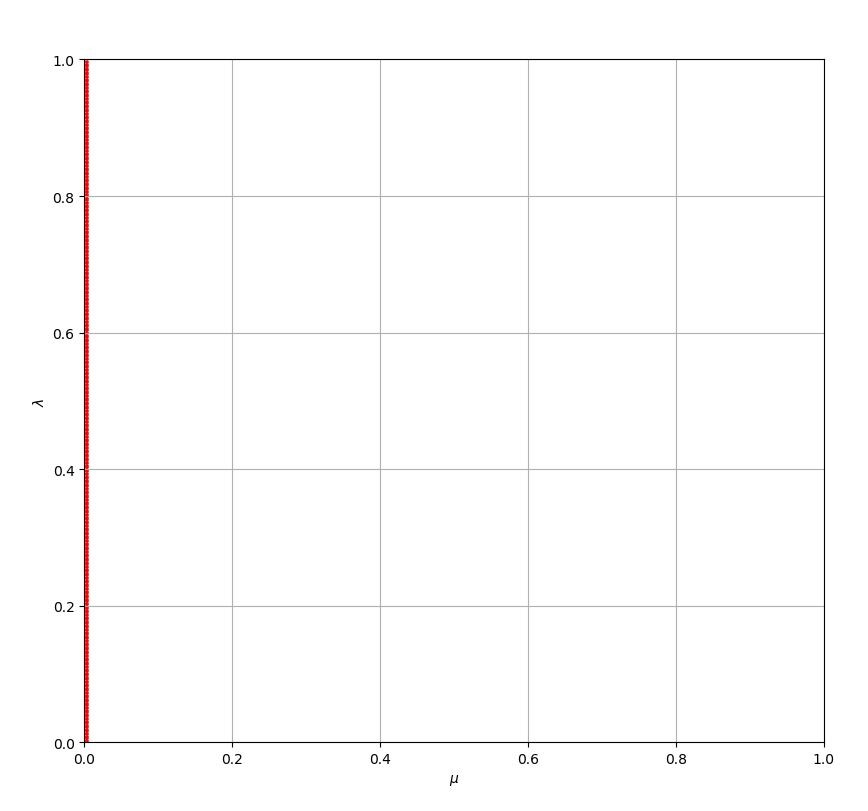
\includegraphics[width=\linewidth]{part_2/graf_3_1}
		\caption{$\mu = 0, \: \lambda \in [0, 1)$}
	\end{subfigure}
	\begin{subfigure}[b]{0.3 \textwidth}
		\includegraphics[width=\linewidth]{part_2/graf_3_2}
		\caption{
			$
			\left[
			\begin{array}{c}
     			\mu=0, \: \lambda = 1 \\
     			\mu=1, \: \lambda = 0
  			\end{array}
			\right.
			$
		}
	\end{subfigure}
	\begin{subfigure}[b]{0.3 \textwidth}	
		\includegraphics[width=\linewidth]{part_2/graf_3_3}
		\caption{
			$
				\mu \in (0,1), \:
				\lambda \in (0, \frac{1 - \mu}{1 + \mu}]
			$		
		}
	\end{subfigure}
	\newline	
	\centering
	\begin{subfigure}[b]{0.3 \textwidth}
		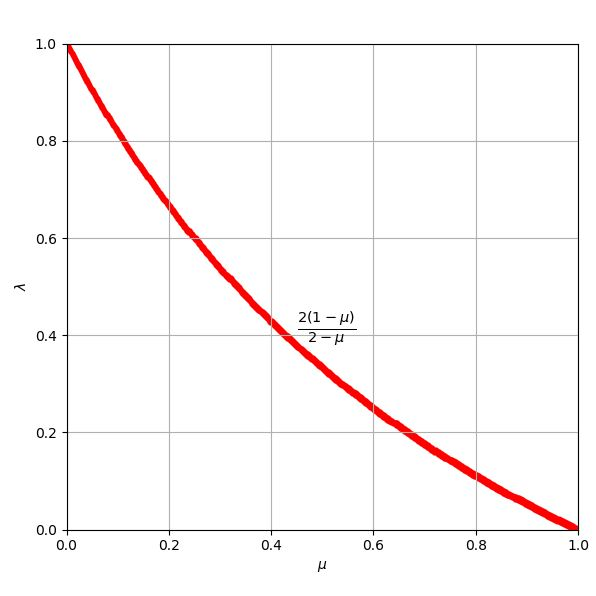
\includegraphics[width=\linewidth]{part_2/graf_3_4}
		\caption{
			$\mu \in (0,1), \lambda = \dfrac{1-\mu}{1+\mu}$		
		}
	\end{subfigure}
	\begin{subfigure}[b]{0.3 \textwidth}
		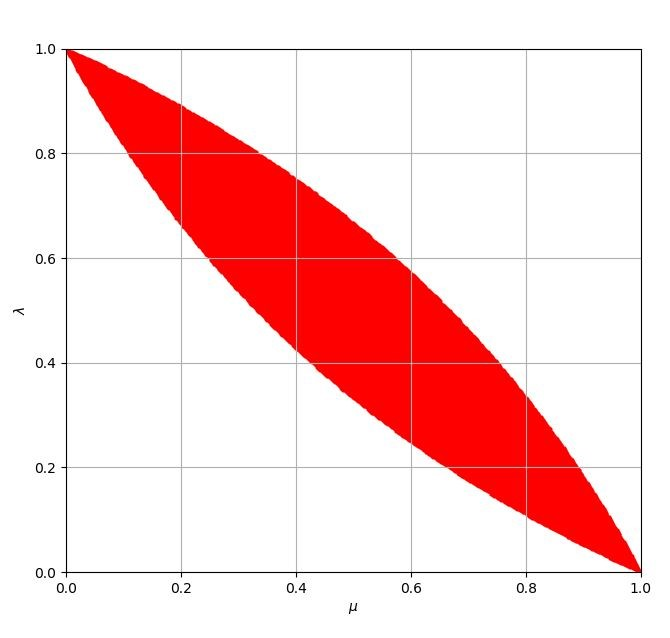
\includegraphics[width=\linewidth]{part_2/graf_3_5}
		\caption{
			$\mu \in [(0, 1), \newline 
			\lambda \in 
			[0, 2\frac{1 - \mu}{2 - \mu}] \cap 
			(\frac{1 - \mu}{1 + \mu}, 1]$
		}
	\end{subfigure}
	\begin{subfigure}[b]{0.3 \textwidth}	
		\includegraphics[width=\linewidth]{part_2/graf_3_6}
		\caption{
			$\mu \in (0, 1), \lambda = 2\dfrac{1 - \mu}{2 - \mu}$: 
		}
	\end{subfigure}
	\newline
	\begin{subfigure}[b]{0.3 \textwidth}
		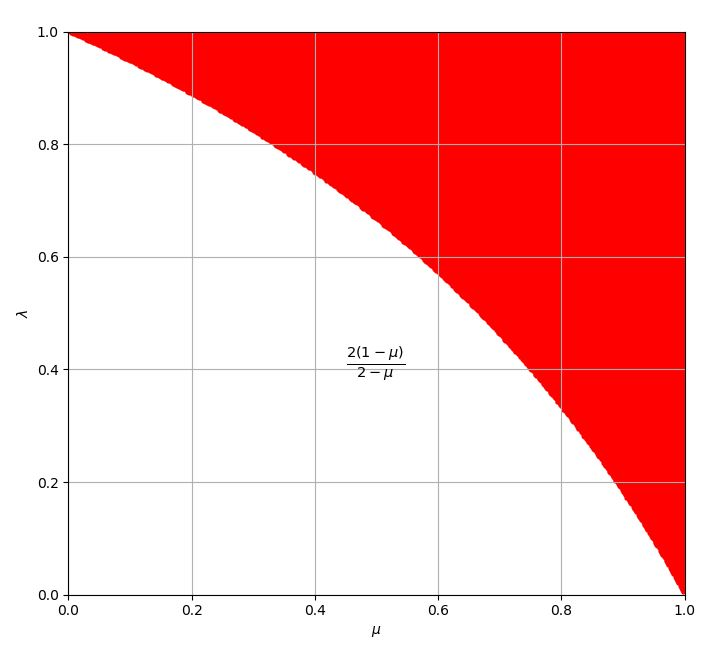
\includegraphics[width=\linewidth]{part_2/graf_3_7}
		\caption{
			$\mu \in (0, 1), 
			\lambda \in (2\frac{1 - \mu}{2 - \mu}, 1]$		
		}
	\end{subfigure}
	\begin{subfigure}[b]{0.3 \textwidth}
		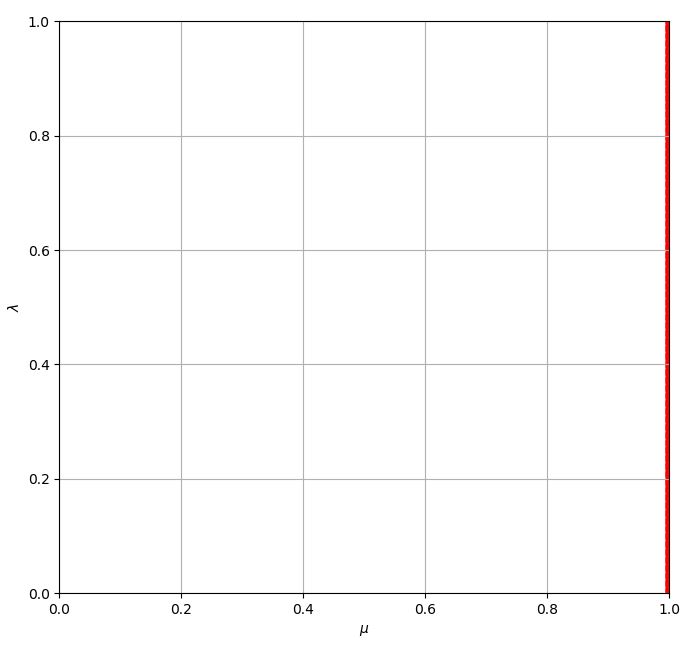
\includegraphics[width=\linewidth]{part_2/graf_3_8}
		\caption{
			$\mu = 1, \lambda \in (0, 1] $		
		}
	\end{subfigure}
	\caption{}
	\label{fig:lambda_mu_set}
\end{figure} % разбито на два файла

	\section{Постановка задачи (значение параметра T=1)}

\subsection{Игровая модель}

\qquad Рассматриваются два игрока - Студент, далее обозначается \textbf{С},
и Преподаватель, далее обозначается \textbf{П}, которые имеют противоположные интересы.
Критерий интересов составляют две велечины, первая из которых является эффективностью
работы \textbf{С} в научной сфере, а второй его эффективностью на подработке.

\textbf{С} выбирает долю $x$ рабочего времени, которую он тратит на подготовку
диплома, оставшееся рабочее время $1-x$ он тратит на подработку. Считается, что производительность \textbf{С} при любых занятий падает с увеличением 
отводимого на них времени, эффективность труда \textbf{С} зададим функцией $\sqrt{x}$
и $\sqrt{1-x}$ соответственно. \textbf{С} может распределять свое время между двумя 
видами деятельности, т.е. имеет множетсво стратегий $x\in X = \{0, 1\}$, 
причём он может использовать смешанные стратегии.

\textbf{П} выбирает - отностится к \textbf{С} требовательно, способствую 
написанию диплома и мешая подработке или же не обращать на него внимания не 
мешая подработке и не помогая с дипломом. \textbf{П} имеет множество стратегий 
$y \in Y=\{1, 2\}$, причём тоже может использовать смешаные стратегии.

\vspace{5mm}
Получаем следующий функциональный критерий:

\begin{equation}
	F(x, y)=
	\big(f_1(x,y), f_2(x,y)\big) =
	\Big(
		\frac{y\sqrt{x}}2,
		\frac{\sqrt{1-x}}y
	\Big)
	\label{eq:player_criterion}
\end{equation}

\qquad \textbf{П} стремится минимизировать (выборая $y \in Y = \{1,2\}$)
критерий $F(x, y)$, а игрок \textbf{С} - максимизировать
 (выбирая $x \in X=[0,1]$).

\vspace{5mm} 
Задачу можно представить в виде многокритериальную игру двух лиц 
с противоположными интересамив 

\begin{equation}
	\bigg \langle F(x,y), X, Y \bigg \rangle, \; y \in Y=\{1, 2\}, \; x \in {X}=[0, 1]
	\label{eq:mc_game}
\end{equation}

\subsection{Постановка зададчи}

Сначала рассмотри случай с параметром $T=1$. Тогда множество $X=\{0, 1\}$.
Игроки используют смешанные стратегии т.е. распределение над своими чистыми стратегиями.
Чистыми стратегиями игроков \textbf{С} и \textbf{П} являются $X=\{0, 1\}$ и $Y=\{1,2\}$ 
соответсвенно. Эти множества дискретны, поэтому распределения задаются в виде векторов 
вида: 

$$(p_1, p_2) \in P = \{(p_1, p_2) \in R_+^2 \; | \; p_1 + p_2 = 1)$$

Множество $Q=P$, введено для наглядности. 
Смешанные стратеги игроков \textbf{С} и \textbf{П} будем обозначать
$q=(q_0,q_1) \in Q$ и $p=(p_0,p_1) \in P$ соответсвенно, причём:

\begin{equation}
\begin{tabu} to 0.9 \textwidth {X[c] X[c]}
	$P(X=0)=q_0$ & $P(Y=1)=p_0$ \\
	$P(X=1)=q_1$ & $P(Y=2)=p_1$ \
	\\
	\end{tabu}	
\label{eq:probability_1}
\end{equation}

Введём обозначения $q := q_1$ и $p := p_1$, тогда $q_0 = 1-q$ и $p_0 = 1 - p$. 
Игрок \textbf{С} использует смешаную стратегию  $(q_0,q_1)$, тогда
его векторный критерий \eqref{eq:player_criterion} приобретает вид: 

$$
	F_\textrm{C}(q,y)=
	\big \langle
		q_0\frac{y\sqrt{0}}{2} + 
		q_1\frac{y\sqrt{1}}{2};
		q_0\frac{\sqrt{1}}{y} +
		q_1\frac{\sqrt{0}}{y}
	\big \rangle 
	= 	
	\big \langle
		\frac{q_1y}{2};
		\frac{q_0}{y}
	\big \rangle 
$$

Игрок \textbf{П} использует смешаную стратегию  $(p_0,p_1)$, тогда
его векторный критерий \eqref{eq:player_criterion} приобретает вид: 

\begin{gather*}
	F_\textrm{П}(x,p)=
	\big \langle 
		(1-p)\frac{1 \cdot \sqrt{x}}{2} + p \frac{2 \cdot \sqrt{x}}{2}; \;
		(1-p)\frac{\sqrt{1-x}}{1}+p\frac{\sqrt{1-x}}{2} 
	\big \rangle=
	\\
	=\frac{1}{2}
	\big \langle
		(p+1)\sqrt{x}; \;
		(2-p)\sqrt{1-x}
	\big \rangle
\end{gather*}
	
\vspace{5mm}

Далее игрок \textbf{С} использует \textit{обратную логическую свёртку}
\eqref{eq:germeyer_scalarization}:

$$
	G(y, q, \mu) = 
	\min \limits_{i: \mu_i > 0} \{\frac{q_1y}{2\mu_0};\frac{q_0}{y\mu_1}\},
$$

a игрок \textbf{П} использует \textit{линейную свёртку}
\eqref{eq:linear_scalarization}:

$$
	L(p, x, \lambda) = 
	\lambda_0 (p+1)\sqrt{x} + \lambda_1 (2-p)\sqrt{1-x}
$$

После чего игрок \textbf{С} осредняет свёртку критерия по стратегиям игрока \textbf{П},
т.е. по переменной $y$:

$$
	\overline G(p,q,\mu)=
	p\min{\{\frac{q}{\mu};
	\frac{1-q}{2(1-\mu)}\}}
	+(1-p)\min\{\frac{q}{2\mu};\frac{1-q}{1-\mu}\},
$$

а игрок \textbf{П} осредняет свёртку критерия по стратегиям игрока \textbf{С},
т.е. по переменной $x$:

$$
	\overline L(p, q, \lambda) =
	\frac{1}{2}\big \{q(3\lambda+p-2)+(2-p)(1-\lambda)\big \}.
$$

Мы установили функции выигрыша игроков. Теперь задачу можно формализовать и представить
как семейство игр двух игроков в нормальный форме:

$$
	\bigg \langle 
		\{\textrm{\textbf{С}, \textbf{П}}\},		
		\{Q, \: P\},		
		\{\overline L(p,q,\lambda), - \overline G(p,q,\mu) \}
	\bigg \rangle 
	, \; (\lambda, \mu) \in \Lambda \times  M
$$

Для нас представляет интерес множество оптимальных точек \eqref{def:optimal_strategy}. % Постановка задачи при параметре
											 % дискретизации Т=2
		\section{Решение игры. \\Параметр дискретизации Т=2}

\subsection{Оптимальная стратегия преподавателя}

Игрок \textbf{П} стремится минимизировать вектор-функцию выигрыша  \eqref{eq:player_criterion}: 
$$
	F(x, y) = \Big \langle
		\frac{y\sqrt{x}}{2},\frac{\sqrt{1-x}}{y}
	\Big \rangle
$$	
Он использует смешанную стратегию, т.е. его стратегией является
распределение $p=(p_0,p_1) \in P$ над множеством чистых стратегий $Y=\{1,2\}$.
Его вектор-функция выигрыша \eqref{eq:player_criterion} приобретает вид:
\begin{multline*}
	F_\textrm{П}(p,x)=
	\big \langle 
		(1-p)\frac{1 \cdot \sqrt{x}}{2} + p \frac{2 \cdot \sqrt{x}}{2}; \;
		(1-p)\frac{\sqrt{1-x}}{1}+p\frac{\sqrt{1-x}}{2} 
	\big \rangle= \\
	=\frac{1}{2}
	\big \langle
		(p+1)\sqrt{x}; \;
		(2-p)\sqrt{1-x}
	\big \rangle.
\end{multline*}
Затем использует \textbf{ЛС} \eqref{eq:linear_scalarization}:
$$
	L(p,x,\lambda)=
	\frac{1}{2}
	\big(
		\lambda(p+1)\sqrt{x} + (1-\lambda)(2-p)\sqrt{1-x}
	\big)
$$
Далее осредняем 
функцию $L(p,x,\lambda)$ по стратегиям противника $x \in X=\{0,\frac{1}{2},1\}$ 
c вероятностями $q=(q_0,q_1,q_2)$:
\begin{multline*} 
	\overline{L}(p,q,\lambda)=
	\frac{1}{2} 
	\Big(
		q_0(1-\lambda)(2-p)\sqrt{1}+
		q_1 \big (\lambda(p+1)\frac{1}{\sqrt{2}} + \\
		+(1-\lambda)(2-p)\frac{1}{\sqrt{2}} \big )+
		q_2\lambda(p+1)\sqrt{1}
	\Big)=
	\\
	=\frac{1}{2\sqrt{2}}
	\Big (
		\big (\lambda(q_1+\sqrt{2}q_2)-(1-\lambda)(q_1+\sqrt{2}q_0) \big)p+
		\big (\lambda(q_1+\sqrt{2}q_2)+2(1-\lambda)(q_1+\sqrt{2}q_0) \big)
	\Big).
\end{multline*}
Функция является линейной по переменной $p$:
$$
	\overline{L}(p,q,\lambda)=k(\lambda,q)p+b(\lambda,q),
$$
где:
\begin{gather*}
	k(q, \lambda) = \frac{1}{2\sqrt{2}}
	\big (\lambda(q_1+\sqrt{2}q_2)-(1-\lambda)(q_1+\sqrt{2}q_0) \big)	,
	\\
	b(q, \lambda) = \frac{1}{2\sqrt{2}}
	\big (\lambda(q_1+\sqrt{2}q_2)+2(1-\lambda)(q_1+\sqrt{2}q_0) \big).
\end{gather*}
Наша задача -- найти 
$p^*(q, \lambda)=\arg \min \limits_{p \in [0, 1]} \overline{L}(p,q,\lambda)$.
Поскольку функция $\overline{L}(p,q,\lambda)$ линейна по переменной 
$p$, следовательно:
$$
	p^*(q, \lambda) =
	\arg \min \limits_{p \in [0, 1]} \overline{L}(p,q,\lambda) =
	\begin{cases}
		0, & k(\lambda,q)>0 \\
		1, & k(\lambda,q)<0 \\
		[0,1], & k(\lambda,q)=0
	\end{cases}	
$$
Рассмотрим функцию $k(q, \lambda)$:
$$
	k(q, \lambda)=\frac{1}{2\sqrt{2}}
	\Big(
		\lambda \big (2+(\sqrt{2}-2)(q_0-q_2) \big) -
		\big (1 - q_2 + (\sqrt{2} - 1)q_0 \big)
	\Big)
$$
Нас интересует знак это функции при различных значениях аргументов.
Введём обозначения:
$$
	\ell(q) = \frac{1 - q_2 + (\sqrt{2} - 1)q_0}{2+(\sqrt{2}-2)(q_0-q_2)}
$$
Напомним, что множество $Q$ имеет следующий вид:
$$
	Q = \{
		(q_0,q_2) \in \mathbb{R}^2_{+} \; | \;
		q_0 + q_2 \leqslant 1
	\}	
$$	
Поскольку для $q \in Q$ верно: 
\begin{gather*}
	2+(\sqrt{2}-2)(q_0-q_2) > 0 
	\\
	1 - q_2 + (\sqrt{2} - 1)q_0 \geqslant 0 
	\\
	q_0 + (\sqrt{2} - 3) q_2 - 1 \leqslant 0
\end{gather*}
Следовательно:
$$
	k(q, \lambda) \vee 0 \Leftrightarrow 
	\lambda \vee \ell(q) \textrm{ где } \vee 
	\textrm{ это один из знаков } >,<,=.
$$
	
Более того верно что 
$\forall \; q \in Q: \; 0 \leqslant \ell(q) \leqslant 1$. 
Проиллюстрируем это на рис. \ref{fig:l}. 
В плоскости $q=(q_0,q_2)$ изображены 
прямые $\ell_1(q)$ и $\ell_2(q)$ такие, что:
\begin{gather*}
	\ell_1(q): \; \ell(q)=0 
	\\
	\ell_2(q): \; \ell(q)=1
\end{gather*}
Зелёным цветом изображена область в которой
$0 \leqslant \ell(q) \leqslant 1$.
Видно, что квадрат $q = [0,1]^2$ а следовательно и
множество $Q$ полностью принадлежит этой области.
\begin{figure}[H]
	\centering
  	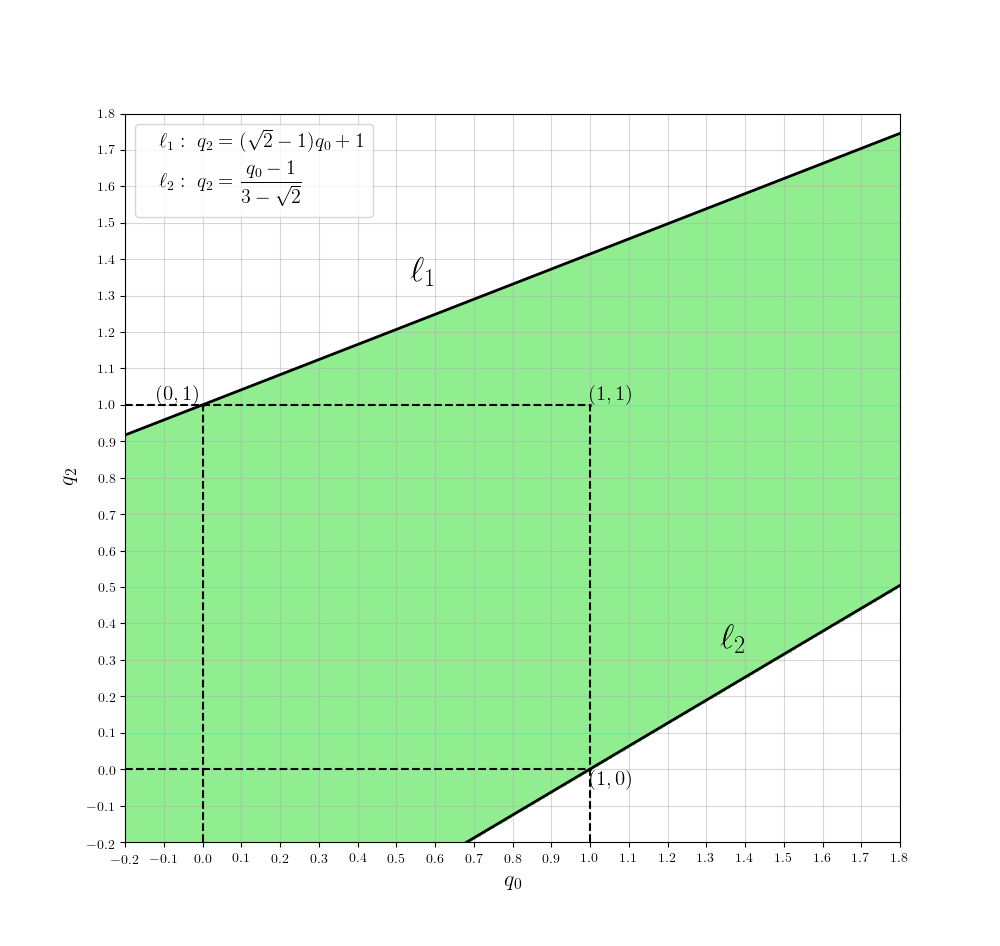
\includegraphics[scale=0.5]{part_3/graf_3_1}
  	\caption{}
  	\label{fig:l}
\end{figure}

Следовательно $\forall \; q=(q_0, q_2) \in Q \;
\exists \; \lambda \in [0,1]: \; k(\lambda,q)=0$.
\begin{equation}
	\label{eq:p*}
	p^*(\lambda,q)=
	\arg \min \limits_{p \in [0, 1]} \overline{L}(p,q,\lambda)=
	\begin{cases}
		0, & \lambda \in \big(\ell (q), 1\big] \\
		1, & \lambda \in \big[0, \ell(q) \big) \\
		[0,1], & \lambda=\ell(q)
	\end{cases},
\end{equation}

где $\ell(q)=\dfrac{1 - q_2 + (\sqrt{2} - 1)q_0}{2+(\sqrt{2}-2)(q_0-q_2)}$. % Решения для Преподователя
		\subsection{Рассмотрим игру за студента}

Игрок \textbf{С} стремится максимизировать вектор-функцию выигрыша: 
$$
	F(x, y) = (\frac{y\sqrt{x}}{2},\frac{\sqrt{1-x}}{y})
$$
Игрок \textbf{С} использует смешанную стратегию, т.е. его стратегией является
распределение $q=(q_0,q_1,q_2)$ над множеством чистых стратегий 
$X=\{0,\frac{1}{2},1\}$:
\begin{gather*}
	F_\textrm{C}=
	\big \langle
		q_0\frac{y\sqrt{0}}{2} + 
		q_1\frac{y}{2} \sqrt{\frac{1}{2}} + 
		q_2\frac{y\sqrt{1}}{2};
		q_0\frac{\sqrt{1}}{y} +
		q_1\frac{1}{y} \sqrt{\frac{1}{2}} +
		q_2\frac{\sqrt{0}}{y}
	\big \rangle = 
	\\
	=\big \langle
		\frac{y}{2}\cdot\frac{1-q_0+(\sqrt{2}-1)q_2}{\sqrt{2}};
		\frac{1}{y}\cdot\frac{1-q_2+(\sqrt{2}-1)q_0}{\sqrt{2}}
	\big \rangle
\end{gather*}
Затем использует \textbf{ОЛС} \eqref{eq:RL_scalarization}. 
Сначала рассмотрим вырожденные случаи для свёртки - когда 
параметры равны $\mu=0$ и  $\mu=1$. 

%-----------------------------------------------------------------------

\textbf{(1)} 
Если $\mu=0$:
$$
	G(y,q,0)=\frac{1}{\sqrt{2}}\cdot \frac{1-q_2+(\sqrt{2}-1)q_0}{y}
$$	

Далеем осредняем функцию $G(y,q,0)$ по стратегиям 
противника $y \in Y=\{1,2\}$ c вероятностями $(1-p,p)$:
\begin{gather*}
	\overline G(p,q,0)=
	\frac{1-p}{\sqrt{2}} \cdot \frac{1-q_2+(\sqrt{2}-1)q_0}{1}+
	\frac{p}{\sqrt{2}} \cdot \frac{1-q_2+(\sqrt{2}-1)q_0}{2}=\\
	=\frac{(2-p)(1-q_2+(\sqrt{2}-1)q_0)}{2\sqrt{2}}
\end{gather*}
	
Найдём частные производную по переменным $q_0$ и $q_2$. 
Введём следующие обозначения для сокращения записи:

\begin{equation}
	\frac{\partial \overline G(p,q,\mu)}{\partial q}=
	\langle 
		\frac{\partial \overline G(p,q,\mu)}{\partial q_0};
		\frac{\partial \overline G(p,q,\mu)}{\partial q_2} 
	\rangle=
	\langle g_1(p,q,\mu), g_2(p,q,\mu) \rangle
	\label{eq:G_dericative}
\end{equation}

$$
	\frac{\partial \overline G(p,q,0)}{\partial q}
	=\frac{2-p}{2\sqrt{2}} \langle \sqrt{2}-1;-1\rangle
$$
Поскольку $p \leqslant 1$, то $\dfrac{2-p}{2\sqrt{2}} > 0 $.
Мы рассматриваем задачу максимизации \\ на множестве $Q$, cледовательно:
$$
	q^* = \arg \max \limits_{q \in Q} \overline G(p,q,0)=(1,0).
$$
	
%--------------------------------------------------------------------
	
\textbf{(2)}
Если $\mu=1:$
$$
	G(y,q,1)=\frac{1}{\sqrt{2}}\cdot \frac{1-q_2+(\sqrt{2}-1)q_0}{y}
$$	
Далеем осредняем функцию $G(y,q,1)$ по стратегиям 
противника $y \in Y=\{1,2\}$ c вероятностями $(1-p,p)$:
\begin{gather*}
	\overline G(p,q,1)=
	\frac{1-p}{\sqrt{2}} \cdot \frac{1-q_0+(\sqrt{2}-1)q_2}{2}+
	\frac{p}{\sqrt{2}} \cdot \frac{1-q_0+(\sqrt{2}-1)q_2}{1}=\\
	=\frac{(p+1)(1-q_0+(\sqrt{2}-1)q_2)}{2\sqrt{2}}
\end{gather*}
Найдём частные производную по переменным $q_0$ и $q_2$:	
$$
	\frac{\partial \overline G(p,q,1)}{\partial q}
	=\frac{p+1}{2\sqrt{2}} \langle -1; \sqrt{2}-1\rangle
$$
Поскольку $p \geqslant 0$, то $\dfrac{p+1}{2\sqrt{2}} > 0 $.
Мы рассматриваем задачу максимизации на множестве $Q$, 
cледовательно:
$$
	q^* = \arg \max \limits_{q\in Q} \overline G(p,q,1)=(0,1).
$$

%--------------------------------------------------------------------

\textbf{(3)} 
Теперь $\mu \neq 0,1$:
$$
	G(y,q,\mu)=\frac{1}{\sqrt{2}}\min \limits_{0<\mu<1}
	\big \langle
		\frac{y}{2} \cdot \frac{1-q_0+(\sqrt{2}-1)q_2}{\mu};
		\frac{1}{y} \cdot \frac{1-q_2+(\sqrt{2}-1)q_0}{1-\mu}
	\big \rangle	
$$
Далеем осредняем функцию $G(y,q,\mu)$ по стратегиям 
противника $y \in Y=\{1,2\}$ c вероятностями $(1-p,p)$:
\begin{multline}
	\label{eq:G_aver}
	\overline G(p,q,\mu)=\frac{1-p}{\sqrt{2}}\min \limits_{0<\mu<1}
	\big \langle
		\frac{1-q_0+(\sqrt{2}-1)q_2}{2\mu};
		\frac{1-q_2+(\sqrt{2}-1)q_0}{1-\mu}
	\big \rangle + \\
	+\frac{p}{\sqrt{2}}\min \limits_{0<\mu<1}
	\big \langle
		\frac{1-q_0+(\sqrt{2}-1)q_2}{\mu};
		\frac{1-q_2+(\sqrt{2}-1)q_0}{2(1-\mu)}
	\big \rangle 
\end{multline}
	
Введём вспомогательные обозначения:
\begin{gather*}
	\ell_1(q,\mu)=\frac{1-q_0+(\sqrt{2}-1)q_2}{2\mu} \\
	\ell_2(q,\mu)=\frac{1-q_2+(\sqrt{2}-1)q_0}{1-\mu} \\
	\ell_3(q,\mu)=\frac{1-q_0+(\sqrt{2}-1)q_2}{\mu} \\
	\ell_4(q,\mu)=\frac{1-q_2+(\sqrt{2}-1)q_0}{2(1-\mu)}
\end{gather*}
	
	
Для различных значений переменной $\mu$ рассмотрим 
взаимные расположения множеств $\ell_1>\ell_2$ и $\ell_3>\ell_4$
на плоскости $(q_0,q_2)$. Другими словами для фиксированного 
значения $\mu \in [0,1]$ найдём области плоскости, в которых 
достигается минимум одного из выражений в \eqref{eq:G_aver}
	
\begin{figure}[H]
   	\centering
    \begin{subfigure}[b]{0.22 \textwidth}
    	\centering
    	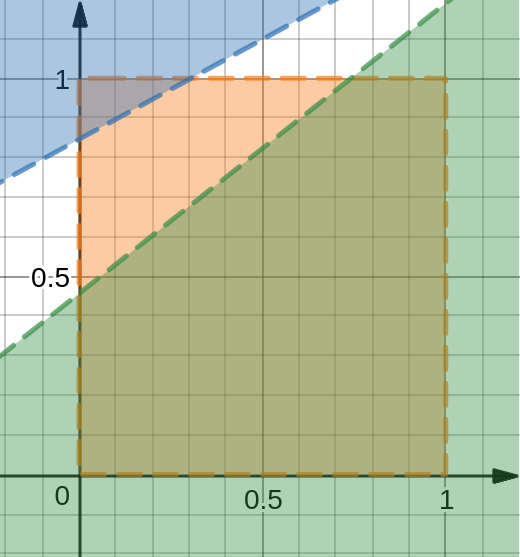
\includegraphics[width=\textwidth]{part_3/graf_6_1}
		\caption{$\mu=0.8$}
        \label{fig:y equals x}
    \end{subfigure}
    \hfill
    \begin{subfigure}[b]{0.22 \textwidth}
       	\centering
       	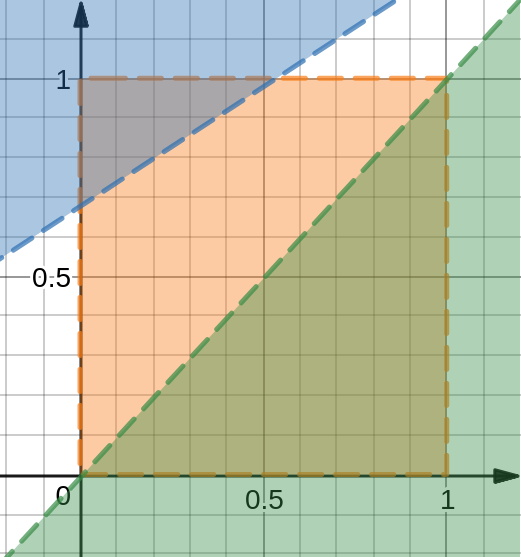
\includegraphics[width=\textwidth]{part_3/graf_6_2}
       	\caption{$\mu=\frac{2}{3}$}
       	\label{fig:three sin x}
     \end{subfigure}
     \hfill
     \begin{subfigure}[b]{0.22 \textwidth}
       	\centering
       	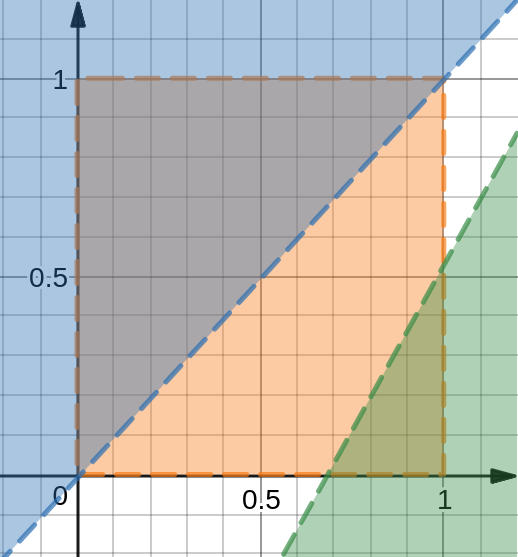
\includegraphics[width=\textwidth]{part_3/graf_6_3}
       	\caption{$\mu=\frac{1}{3}$}
       	\label{fig:five over x}
     \end{subfigure}
     \hfill
     \begin{subfigure}[b]{0.22 \textwidth}
       	\centering
       	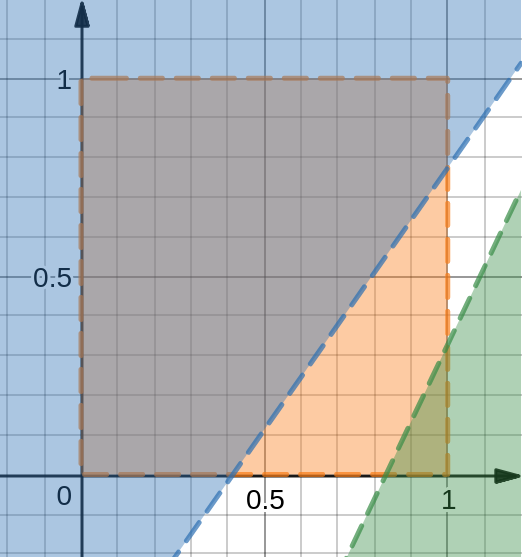
\includegraphics[width=\textwidth]{part_3/graf_6_4}
		\caption{$\mu=0.1$}
        \label{fig:five over x}
     \end{subfigure}
\end{figure}
Поясним график. Синяя область -- это множество $\ell_1 > \ell_2$.
Зелёная область на графике -- это множнство $\ell_3 < \ell_4$.
Область между ними -- это множество $\{\ell_1<\ell_2 \cap \ell_3 > \ell_4\}$.
Исходя из графиков $\{\ell_1>\ell_2 \cap \ell_3 < \ell_4\} = \emptyset$ 
при $(\mu, q) \in (0, 1) \times [0, 1]^2$.
Поскольку граничные случаи для параметра $\mu$ были рассмотрены в первых
двух пунктах, то квадрат $[0,1]^2$ на плоскости $(q_0,q_2)$ делится на 3
связные, не пересекающихся множества.
	
\textbf{Добавить доказательство того, что всего три возможных варианта}\\
\textbf{(1)} 
Рассмотрим полуплоскость, которая определяется системой
$
	\begin{cases}
		\ell_1 > \ell_2 \\
		\ell_3 > \ell_4
	\end{cases}.
$
Вторая строчка в системе является избыточной, т.к. следует из первой.
Система эквивалентна неравенству $\ell_1 > \ell_2$. Выражение \eqref{eq:G_aver} на этом множестве принимает следующий вид:
\begin{gather*}
	\overline G(p,q,\mu)=
	\frac{1-p}{\sqrt{2}} \cdot \frac{1-q_2+(\sqrt{2}-1)q_0}{1-\mu} + 
	\frac{p}{\sqrt{2}} \cdot \frac{1-q_2+(\sqrt{2}-1)q_0}{2(1-\mu)} = \\
	=\frac{2-p}{2\sqrt{2}}\cdot\frac{1-q_2+(\sqrt{2}-1)q_0}{1-\mu}		
\end{gather*}
\textbf{(2)}
Рассмотрим полуплоскость, которая определяется системой
$
	\begin{cases}
		\ell_1 < \ell_2 \\
		\ell_3 < \ell_4
	\end{cases}.
$
Первая строчка в системе является избыточной, т.к. следует из второй.
Система эквивалентна неравенству $\ell_3 < \ell_4$.
Выражение \eqref{eq:G_aver} на этом множестве принимает следующий вид
\begin{gather*}
	\overline G(p,q,\mu)=
	\frac{1-p}{\sqrt{2}} \cdot \frac{1-q_0+(\sqrt{2}-1)q_2}{2\mu} + 
	\frac{p}{\sqrt{2}} \cdot \frac{1-q_0+(\sqrt{2}-1)q_2}{\mu} = \\
	=\frac{1+p}{2\sqrt{2}}\cdot\frac{1-q_0+(\sqrt{2}-1)q_2}{\mu}		
\end{gather*}
\textbf{(3)}
Рассмотрим область, которая определяется системой
$
	\begin{cases}
		\ell_1 < \ell_2 \\
		\ell_3 > \ell_4
	\end{cases}.
$
Выражение \eqref{eq:G_aver} на этом множестве принимает следующий вид:	
\begin{gather*}	
	\overline G(p,q,\mu)=
	\frac{1-p}{\sqrt{2}} \cdot \frac{1-q_0+(\sqrt{2}-1)q_2}{2\mu} +
	\frac{p}{\sqrt{2}} \cdot \frac{1-q_2+(\sqrt{2}-1)q_0}{2(1-\mu)}=
	\\	
	=\frac{(1-p)(1-\mu)(1-q_0+(\sqrt{2}-1)q_2)+p\mu(1-q_2+(\sqrt{2}-1)q_0)}
	{2\sqrt{2}\mu(1-\mu)}
\end{gather*}
	
Итого: 

$$
	\overline G(p,q,\mu) =		
	\begin{cases}
		\dfrac{2-p}{2\sqrt{2}}\cdot\dfrac{1-q_2+(\sqrt{2}-1)q_0}{1-\mu} 
		,\hspace{2mm} \ell_1 \geqslant \ell_2		
		\\
		\dfrac{1+p}{2\sqrt{2}}\cdot\dfrac{1-q_0+(\sqrt{2}-1)q_2}{\mu}
		,\hspace{2mm} \ell_3 \leqslant \ell_4\\
		\dfrac{(1-p)(1-\mu)(1-q_0+(\sqrt{2}-1)q_2)+p\mu(1-q_2+(\sqrt{2}-1)q_0)}
		{2\sqrt{2}\mu(1-\mu)}
		, \textrm{ иначе}
	\end{cases}
$$	
Тогда вектор производных по переменным $(q_0,q_2)$ имеет вид:
$$
	\frac{\partial \overline{G}(p,q,\mu)}{\partial q}=
	\begin{cases}
		\dfrac{2-p}{2\sqrt{2}(1-\mu)} \langle \sqrt{2}-1; -1 \rangle 
 		,\hspace{2mm}
 		\ell_1 \geqslant \ell_2\\
		
		\dfrac{1+p}{2\sqrt{2}\mu} \langle -1; \sqrt{2}-1 \rangle
		,\hspace{2mm}
		\ell_3 \leqslant \ell_4\\
		\textbf{g}(p,\mu)
		,\hspace{2mm}
		\begin{cases}
			\ell_1 \leqslant \ell_2\\
			\ell_3 \geqslant \ell_4\\
		\end{cases}
	\end{cases}
$$
где:
$$
	\textbf{g}(p,\mu) =
	\dfrac{1}{2\sqrt{2}\mu(1-\mu)}
	\big \langle 
		(\sqrt{2} - 1)p\mu -(1-p)(1-\mu);
		(\sqrt{2} - 1)(1-p)(1-\mu) - p\mu			
	\big \rangle
$$
	
%------------------------------------------------------------

\textbf{(1)}
Рассмотрим $\ell_1 \geqslant \ell_2$. Тогда вектор производных 
по переменным $(q_0,q_2)$ имеет вид:
$$
	\frac{\partial \overline{G}(p,q,\mu)}{\partial q}=
	\frac{2-p}{2\sqrt{2}(1-\mu)} \langle \sqrt{2}-1; -1 \rangle
$$	
Введём вспомогалетльную функцию 
$\ell_B(q, \mu):=(\ell_1-\ell_2) \cdot \mu(1-\mu)$,
множество, на котором она принимает неотрицательные значения 
составляют интересующую нас область. Множитель $\mu(1-\mu)$ является строго
положительным на $\mu \in (0,1)$, поэтому не влияет на знак. Функция
является линейной по переменным $q_0$ и $q_2$:
 
$$
	\ell_B(q, \mu) = 
	(1+\mu(2\sqrt{2}-3))q_0+
	(1-\sqrt{2}+\mu(\sqrt{2}-3))q_2
	+3\mu-1
$$ 	
Параметр $\mu$ изменяется в диапазоне $(0,1)$, причём:
\begin{gather*}	
	\ell_B(q,\mu) \xrightarrow[\mu\rightarrow 1]{} 
	1-q_0+(\sqrt{2}-1)q_2\\	
	\ell_B(q,\mu) \xrightarrow[\mu\rightarrow 0]{} 	
	1-q_2+(\sqrt{2}-1)q_0
\end{gather*}
Предельные положения $\ell_B(q, \mu)=0$ изображены на графике 
\eqref{fig:l_B_limits}.

\begin{figure}[H]
	\centering
  	\includegraphics[scale=0.5]{part_3/graf_3_2}
  	\caption{}
  	\label{fig:l_B_limits}
\end{figure}
Найдём значение $\mu$, при котором прямая $\ell_B(q, \mu)$ проходит через точку
$q=(0,0)$:
$$
	\ell_B(0,0,\hat \mu) = 0
	\Rightarrow \hat \mu = \frac{1}{3}
$$	
	
Очевидно, что на полиэдре $P_B(\mu):$
		
$$
	P_B(\mu)=\{q \in Q \; | 
	\;  \ell_B(q, \mu) \geqslant 0 \}, \; \mu \in (0,1),
$$
	
функция $\overline{G}(p,q,\mu)$ достигает максимума в точке $B(\mu):$
$$
	q^* = \arg \max \limits_{q\in P_B(\mu)} \overline G(y,q,\mu) = B(\mu)=
	\begin{cases}
		(0, q_2) : \ell_B(0,q_2,\mu)=0, & \frac{1}{3} \leqslant \mu < 1 \\
		(q_0, 0) : \ell_B(q_0,0,\mu)=0, & 0 < \mu \leqslant \frac{1}{3} \\
	\end{cases}	
$$

\begin{figure}[H]
   	\centering
	\begin{subfigure}[b]{0.4 \textwidth}
        \centering
        \includegraphics[width=\textwidth]{part_3/graf_3_3}
        \caption{$\mu=0.1 < \frac{1}{3}$}
         \label{fig:y equals x}
     \end{subfigure}
     \hspace{10mm}
     \begin{subfigure}[b]{0.4 \textwidth}
       	\centering
       	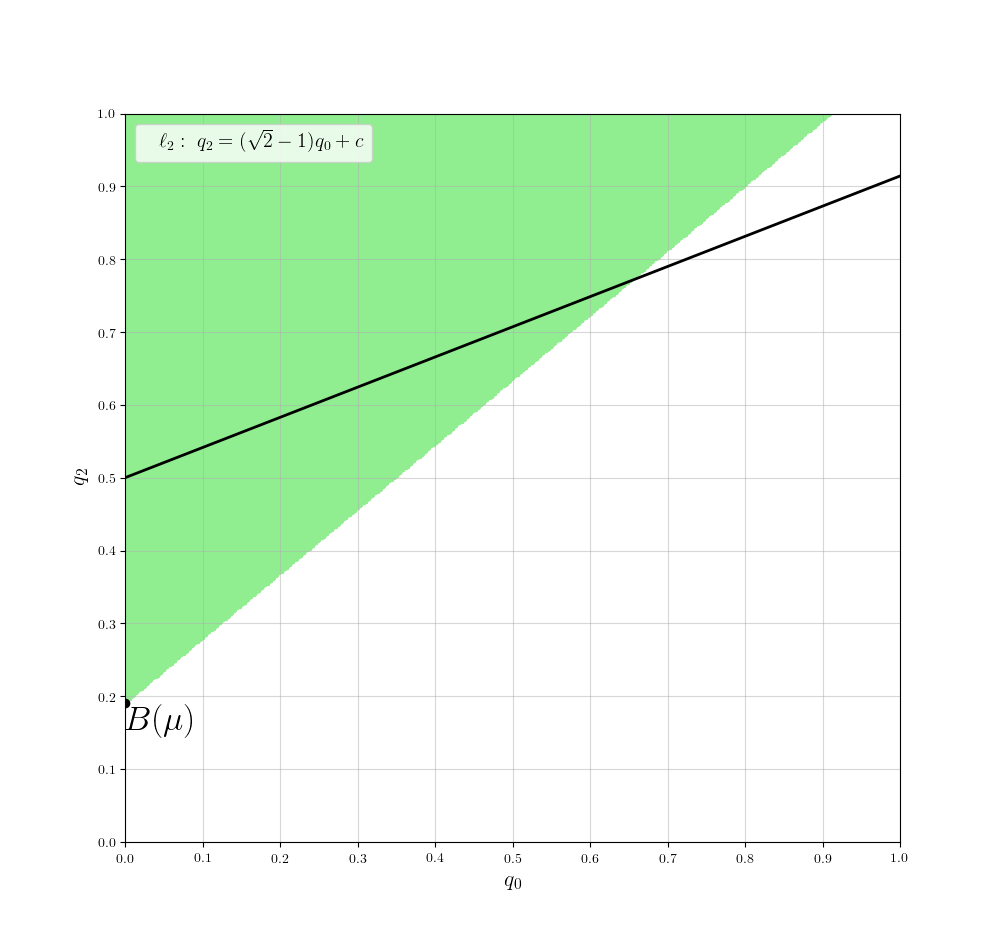
\includegraphics[width=\textwidth]{part_3/graf_3_4}
       	\caption{$\mu=0.4 > \frac{1}{3}$}
       	\label{fig:three sin x}
     \end{subfigure}
\end{figure}	

На графике зелёным цветом изображена область $P_B(\mu)$, чёрным цветом
обозначены линии уровня и стрелкой соответсвенно градиент функции.
Рассмотрим эти два случая и найдём явное выражение для точки $B(\mu)$:
	
\textbf{(a)}
Если $\frac{1}{3} \leqslant \mu \leqslant 1$ то координата $q_2$ 
точки максимума определяется из условия: 	
\begin{gather*}
	\ell_B(0,q_2,\mu)=0
	\\
	(1-\sqrt{2}+\mu(\sqrt{2}-3))q_2+3\mu-1=0
	\hspace{3mm} \Rightarrow \hspace{3mm}
	q_2=\frac{3\mu-1}{\sqrt{2}-1+(3-\sqrt{2})\mu}	
	\\
	q^*=(0;\dfrac{3\mu-1}{\sqrt{2}-1+(3-\sqrt{2})\mu}), \hspace{3mm}
	\frac{1}{3} \leqslant \mu \leqslant 1
\end{gather*}

\textbf{(b)}
Если $0 \leqslant \mu \leqslant \frac{1}{3}$ то координата $q_0$ точки 
максимума определяется из условия: 	
\begin{gather*}
	\ell_B(q_0,0,\mu)=0
	\\	
	(1+\mu(2\sqrt{2}-3))q_0
	+3\mu-1=0
	\hspace{3mm} \Rightarrow \hspace{3mm}
	q_0=\frac{1-3\mu}{1+(2\sqrt{2}-3\mu)}	
	\\ 	
	q^*=(\frac{1-3\mu}{1+(2\sqrt{2}-3\mu)}; 0), \hspace{3mm}
	0 \leqslant \mu \leqslant \frac{1}{3}
\end{gather*}
Следовательно:
\begin{equation} 
	\label{eq:B_point}
	B(\mu) = \arg \max \limits_{q\in P_B(\mu)} \overline G(y,q,\mu) = 
	\begin{cases}
		(0;\dfrac{3\mu-1}{\sqrt{2}-1+(3-\sqrt{2})\mu})
		, & \frac{1}{3} \leqslant \mu \leqslant 1
		\\
		(\dfrac{1-3\mu}{1+(2\sqrt{2}-3\mu)};0)
		, & 0 \leqslant \mu \leqslant \frac{1}{3}
	\end{cases}
\end{equation}

%------------------------------------------------------------

\textbf{(2)} Рассмотрим $\ell_3 \leqslant \ell_4$.
Производная в области имеет вид:
	
$$
	\frac{\partial \overline{G}(p,q,\mu)}{\partial q}=
	\frac{1+p}{2\sqrt{2}\mu} \langle -1;\sqrt{2}-1 \rangle 
$$
 	
Введём вспомогалетльную функцию	
$\ell_A(q, \mu):=(\ell_3-\ell_4) \cdot \mu(1-\mu)$,
множество, на котором она принимает неотрицательные значения 
составляют интересующую нас область. Множитель $\mu(1-\mu)$ является строго
положительным на $\mu \in (0,1)$, поэтому не влияет на знак. Функция
является линейной по переменным $q_0$ и $q_2$:
 	
$$
	\ell_A(q, \mu)=
	-(2+(\sqrt{2}-3)\mu)q_0
	-(2-2\sqrt{2}+(2\sqrt{2}-3)\mu)q_2
	-3\mu+2
$$ 	
 	
Параметр $\mu$ изменяется в диапазоне $(0,1)$, причём	
	
\begin{gather*}	
	\ell_A(q,\mu) \xrightarrow[\mu\rightarrow 1]{} 
	1-q_0+(\sqrt{2}-1)q_2\\	
	\ell_A(q,\mu) \xrightarrow[\mu\rightarrow 0]{} 	
	1-q_2+(\sqrt{2}-1)q_0\\
\end{gather*}
	
	Предельные положения $\ell_B(q, \mu)=0$ изображены на графике \eqref{fig:l_B_limits}.
	Найдём значение $\mu$ при котором прямая 
	$\ell(q, \mu)$ проходит через точку
	$q=(0,0)$:
	
	$$\ell_A(0,0,\hat \mu) = 0 \Rightarrow \hat \mu = \frac{2}{3}$$
	
	Очевидно, что на полиэдре $P_2(\mu):$
	
	$$P_A(\mu)=\{q \in Q \; | 
	\;  \ell_3(q, \mu) \leqslant \ell_4(q, \mu) \}, \; \mu \in (0,1)$$
	
	функция $\overline{G}(p,q,\mu)$ достигает максимума в точке $A(\mu):$
	
	\begin{gather*}
		A(\mu)= \arg \max \limits_{q\in P_A(\mu)} \overline G(p,q,\mu) =
		\begin{cases}
			(0, q_2) : \ell_A(0,q_2,\mu)=0, & \frac{2}{3} \leqslant \mu \leqslant 1 \\
			(q_0, 0) : \ell_A(q_0,0,\mu)=0, & 0 \leqslant \mu \leqslant \frac{2}{3} \\
		\end{cases}		
	\end{gather*}
	
	\begin{figure}[H]
    	\centering
     	\begin{subfigure}[b]{0.45 \textwidth}
        	\centering
        	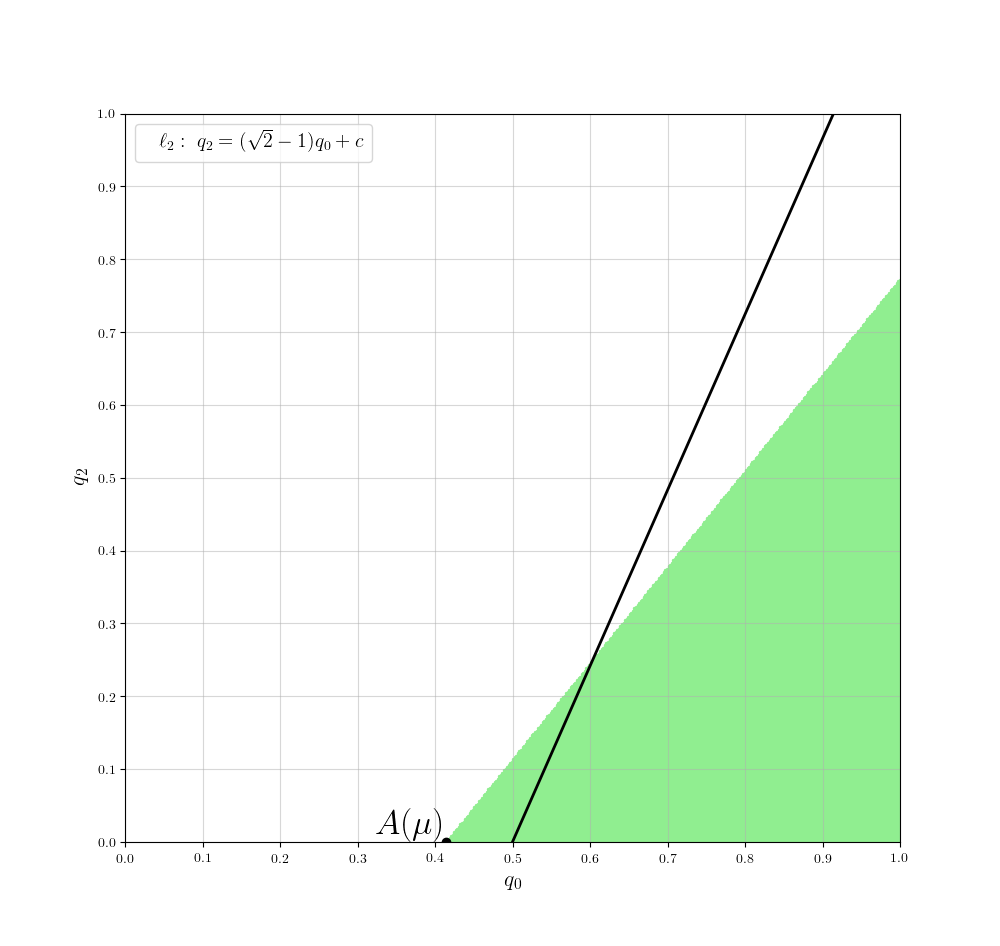
\includegraphics[width=\textwidth]{part_3/graf_3_5}
        	\caption{$\mu=0.1 < \frac{2}{3}$}
         	\label{fig:y equals x}
     	\end{subfigure}
     	\hspace{10mm}
     	\begin{subfigure}[b]{0.45 \textwidth}
        	\centering
        	\includegraphics[width=\textwidth]{part_3/graf_3_6}
        	\caption{$\mu=0.8 > \frac{2}{3}$}
        	\label{fig:three sin x}
     	\end{subfigure}
	\end{figure}	
	
	На графике зелёным цветом изображена область $P_A(\mu)$, чёрным цветом
	обозначены линии уровня и стрелкой соответсвенно градиент функции.
	Рассмотрим эти два случая и найдём явное выражение для точки $A(\mu)$:

	\textbf{(a)} Если $\frac{2}{3} \leqslant \mu \leqslant 1$ то координата $q_2$ точки 
	максимума определяется из условия: 	
	
	\begin{gather*}	
		\ell_A(0,q_2,\mu)=0 
		\\
		-(2-2\sqrt{2}+(2\sqrt{2}-3)\mu)q_2
		-3\mu+2=0
		\hspace{3mm} \Rightarrow \hspace{3mm}
		q_2=\frac{3\mu-2}{2(\sqrt{2}-1)+(3-2\sqrt{2})\mu}	
		\\
		q^*= (0;\dfrac{3\mu-2}{2(\sqrt{2}-1)+(3-2\sqrt{2})\mu}), 
		\hspace{5mm} \frac{2}{3} \leqslant \mu \leqslant 1
	\end{gather*}


	\textbf{(b)} Если $0 \leqslant \mu \leqslant \frac{2}{3}$ то координата $q_0$ точки 
	максимума определяется из условия: 	
	
	\begin{gather*}
		\ell_A(q_0,0,\mu)=0	
		\\
		-(2+(\sqrt{2}-3)\mu)q_0
		-3\mu+2=0	
		\hspace{3mm} \Rightarrow \hspace{3mm}
		q_0=\frac{2-3\mu}{2+(\sqrt{2}-3)\mu}	
		\\
		q^*= (\dfrac{2-3\mu}{2+(\sqrt{2}-3)\mu};0), 
		\hspace{5mm} 0 \leqslant \mu \leqslant \frac{2}{3}	
	\end{gather*}
	
	Следовательно:
	\begin{equation} \label{eq:A}
		A(\mu) = \arg \max \limits_{q\in P_A(\mu)} \overline G(p,q,\mu) = 
		\begin{cases}
			(0;\dfrac{3\mu-2}{2(\sqrt{2}-1)+(3-2\sqrt{2})\mu})
			, & \frac{2}{3} \leqslant \mu \leqslant 1 \\
			(\dfrac{2-3\mu}{2+(\sqrt{2}-3)\mu};0), & 0 \leqslant \mu \leqslant \frac{2}{3}	
		\end{cases}
	\end{equation}

%------------------------------------------------------------

	\textbf{(3)} Рассмотрим область в которой
	$\begin{cases}
		\ell_1 \leqslant \ell_2 \\	
		\ell_3 \geqslant \ell_4 \\
	\end{cases}	
	$
	
	Частные производные имеют следующий види в данной области.
	
	$
	\dfrac{\partial \overline{G}(p,q,\mu)}{\partial q}=
	\dfrac{1}{2\sqrt{2}\mu(1-\mu)}
	\big \langle 
		(\sqrt{2} - 1)p\mu -(1-p)(1-\mu);
		(\sqrt{2} - 1)(1-p)(1-\mu) - p\mu			
	\big \rangle
	$

	\begin{gather*}
	g_1=(\sqrt{2} - 1)p\mu -(1-p)(1-\mu) \\
	g_2=(\sqrt{2} - 1)(1-p)(1-\mu) - p\mu
	\end{gather*}

 	Заметим, что функция $\overline{G}(p,q,\mu)$
 	является линейной по переменным $q_0$ и $q_2$ т.е.:

	\begin{gather*}
	\overline{G}(p,q,\mu)=g_0(p,\mu) \: q_0+g_2(p,\mu) \: q_2+c(p,\mu)
	\\
	\textrm{и}
	\\
	\overline{G}(p,q,\mu) = 0 \sim q_2 = k(p, \mu) \cdot q_0 + c(p, \mu)	
	\end{gather*}
	
	Рассматриваем функцию на полиэдре $P_{AB}(\mu):$
	
	$$P_{AB}(\mu)=
	\{
		q \in Q \; | \;  
		\ell_A(q, \mu) \geqslant 0 \cap
	 	\ell_B(q, \mu) \leqslant 0
	\},\; \mu \in (0,1) $$

	Ограничение $\ell_A(q, \mu) = 0$ и $\ell_B(q, \mu) = 0$ представимы в 
	эквивалентном виде:
	
	$$\ell_A(q,\mu)=0 \sim \; q_2=k_A(\mu)q_0+c_A(\mu)$$
	$$\ell_B(q,\mu)=0 \sim \; q_2=k_B(\mu)q_0+c_B(\mu)$$

	
	\begin{figure}[H]
		\centering
  		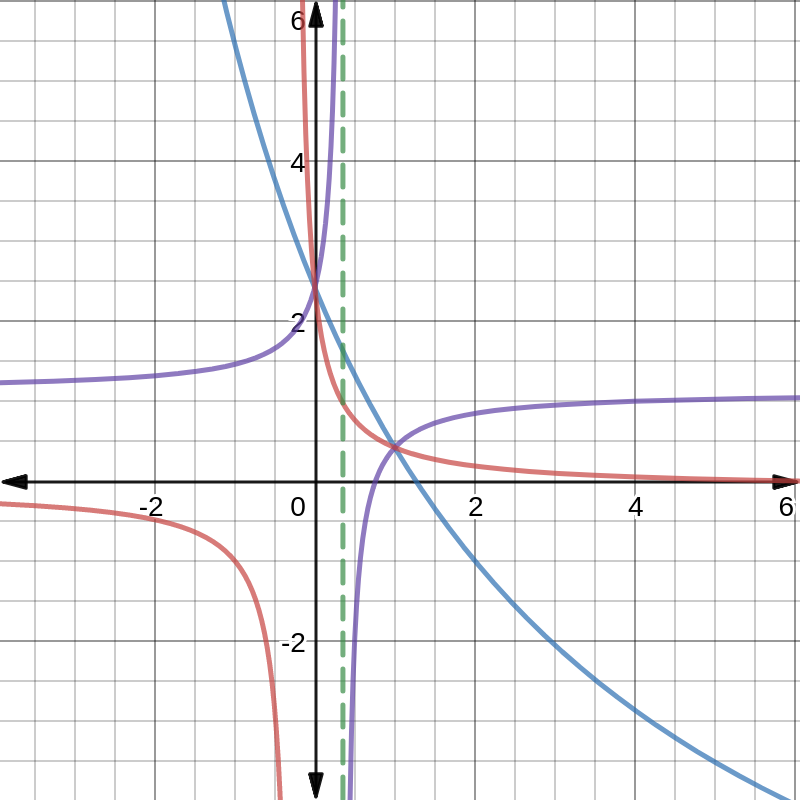
\includegraphics[scale=0.3]{part_3/graf_3_10}
  		\caption{Коэффициенты $k_A(\mu)$, $k_B(\mu)$ и $k(p,\mu)$ при фиксированном $p$}
		\label{fig:k_A,k_B,k}	
	\end{figure}	
	
	Рассмотрим график \ref{fig:k_A,k_B,k}, на котором изображены значения коэффициетов
	при фиксированном значении $p \in [0,1]$. $k_B(\mu)$ изображены красной кривой,
	$k_A(\mu)$ синей и фиолетовой - кривая $k(p, \mu)$. Пунктирная вертикальная линия
	обозначает точку $x$ в которой выражение $g_1=0$. Имеет место неравенство 
	$k_A(\mu) > k_B(\mu)$ при $\mu \in (0,1)$.
	
	$$
	\begin{cases}
	k(\mu) < k_B(\mu) \textrm{ при } g_1(\mu,p) < 0  \\
	k(\mu) > k_A(\mu) \textrm{ при } g_1(\mu,p) > 0 \\
	\end{cases}		
	$$	
	
	
	Следовательно точки максимума функции $\overline{G}(p,q,\mu)$ при фикисированных
	значениях $\mu$ и $p$ могут быть точки: 
	$\{A\}, \{B\}, (0,0)$ и отрезки $[B, A], [0, A], [0,B]$. Где точки
	$A(\mu)$ и $B(\mu)$ определны в \ref{eq:A} и \ref{eq:B}. 
	Рассмотрим три подслучая:
	
	\newpage

	\textbf{(a)} $0 \leqslant \mu \leqslant \frac{1}{3}$. 	
		
	\begin{figure}[H]
    	\centering
     	\begin{subfigure}[b]{0.3 \textwidth}
        	\centering
        	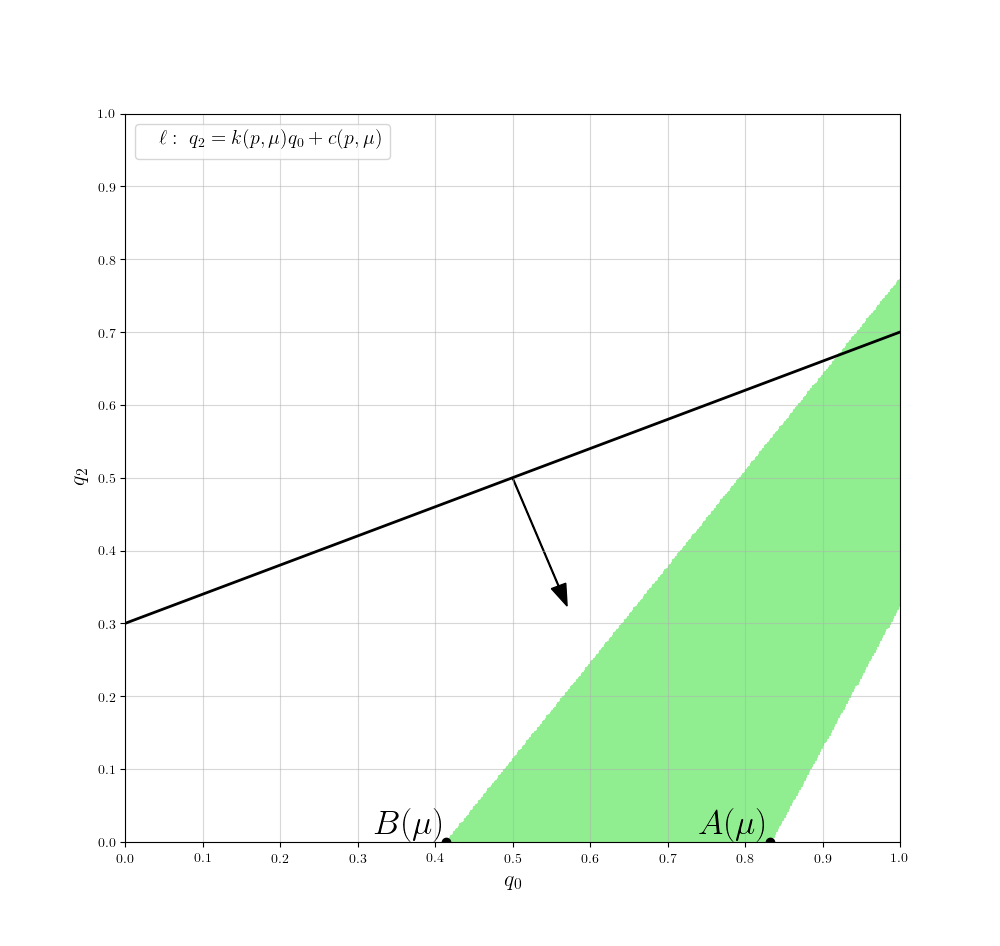
\includegraphics[width=\textwidth]{part_3/graf_3_9_0}
        	\caption{$g_1 > 0 \Rightarrow q^*=A$}
         	\label{fig:y equals x}
     	\end{subfigure}
     	\begin{subfigure}[b]{0.3 \textwidth}
        	\centering
        	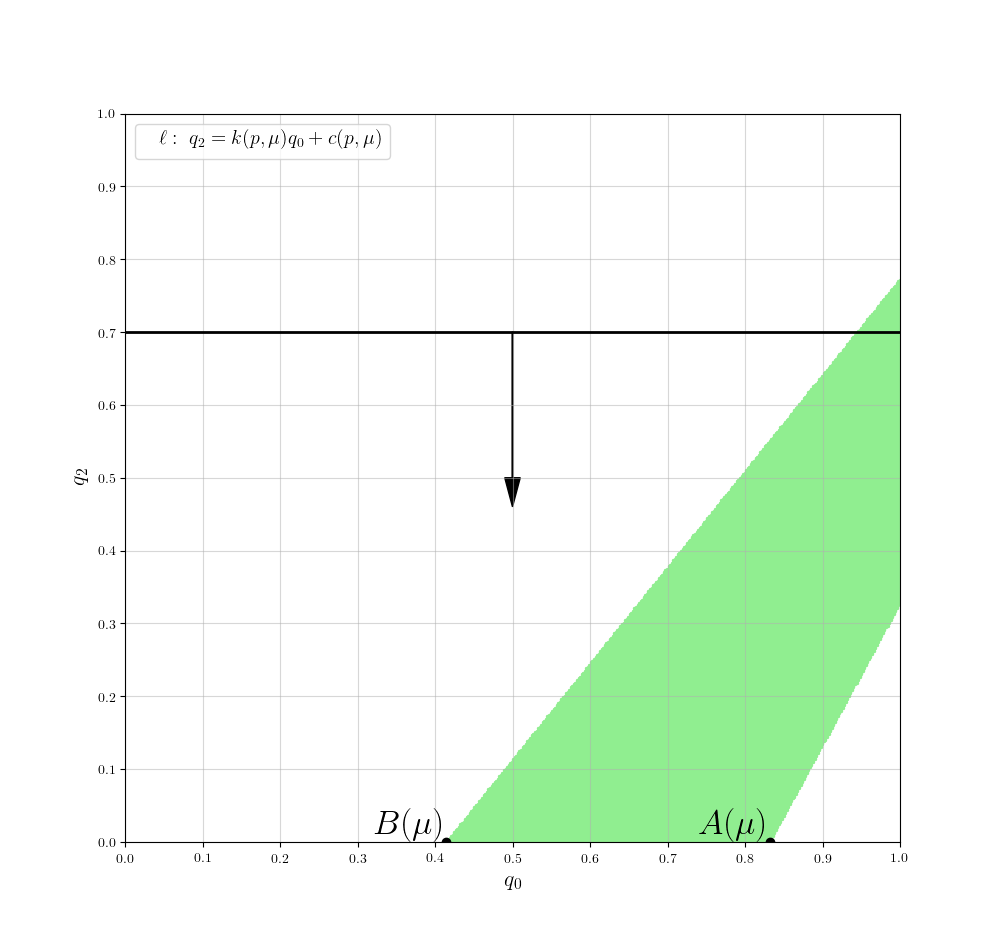
\includegraphics[width=\textwidth]{part_3/graf_3_9_2}
        	\caption{$g_1 = 0 \Rightarrow q^*=[B,A]$}
        	\label{fig:three sin x}
     	\end{subfigure}
     	\begin{subfigure}[b]{0.3 \textwidth}
        	\centering
        	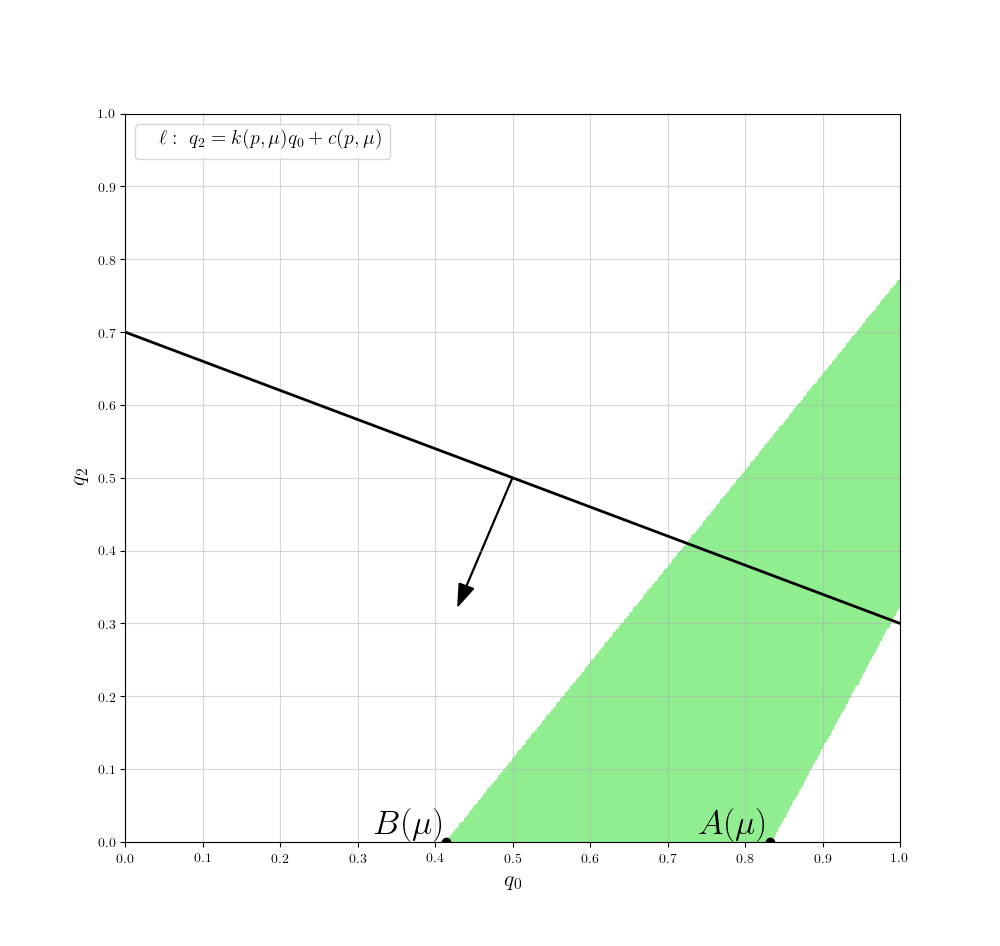
\includegraphics[width=\textwidth]{part_3/graf_3_9_1}
        	\caption{$g_1 < 0 \Rightarrow q^*=B$}
        	\label{fig:three sin x}
     	\end{subfigure}
     	\caption{}
     	\label{fig:3_mu_0}
	\end{figure}

	%Если наклон касательной меньше $k_A$ но больше нуля, то оптимальной точкой
	%является точка $A(\mu)$, если касатальеная паралельна оси $Oq_0$,
	%то множеству оптимальных точек соответсвует отрезок $[B,A]$, если же наклон
	%отрицательный то оптимальной точкой является точка $B(\mu)$.
	%Итого оптимальные точки соответсвуют следующей системе:	
	
	$$
		\begin{cases}
			g_1 > 0 \Rightarrow q^*=A \\
			g_1 = 0 \Rightarrow q^*=[B,A] \\
			g_1 < 0 \Rightarrow q^*=B
		\end{cases}
	$$	
	
	\textbf{(b)} $\frac{2}{3} \leqslant \mu \leqslant 1$
			
	\begin{figure}[H]
    	\centering
     	\begin{subfigure}[b]{0.3 \textwidth}
        	\centering
        	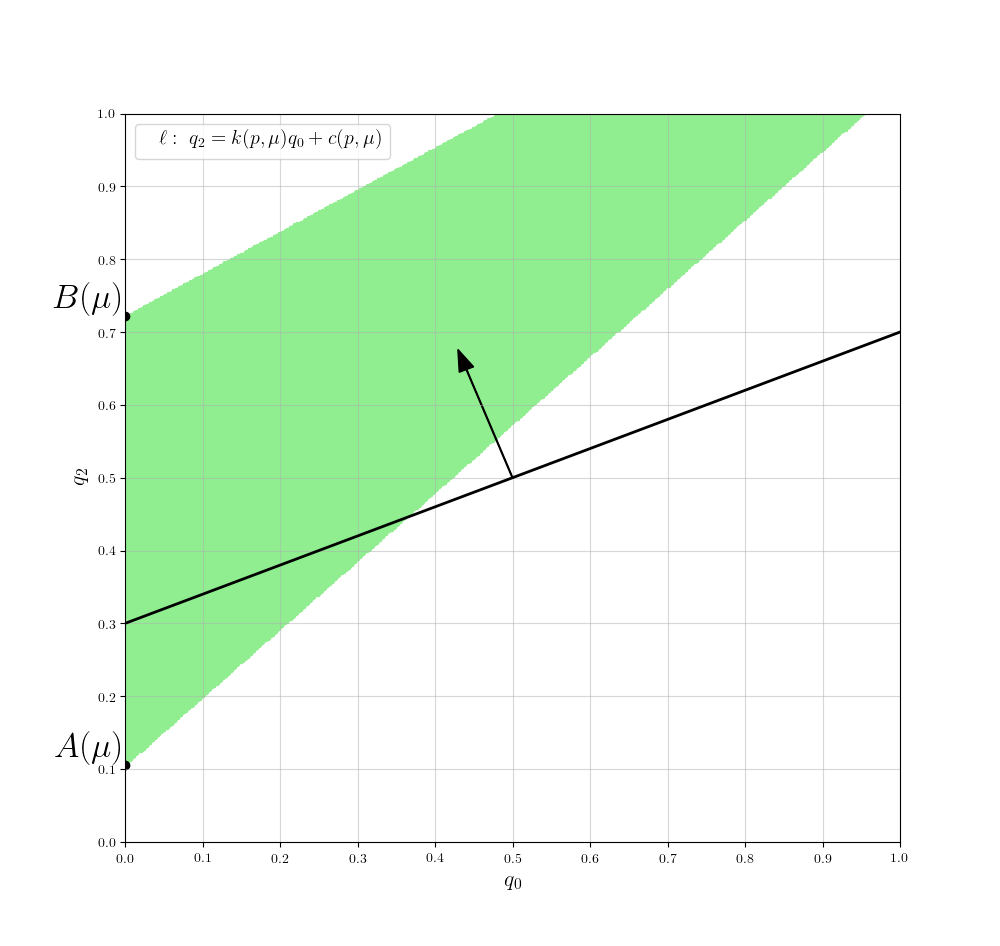
\includegraphics[width=\textwidth]{part_3/graf_3_7_0}
        	\caption{$g_2 > 0 \Rightarrow q^*=B$}
         	\label{fig:y equals x}
     	\end{subfigure}
     	\begin{subfigure}[b]{0.3 \textwidth}
        	\centering
        	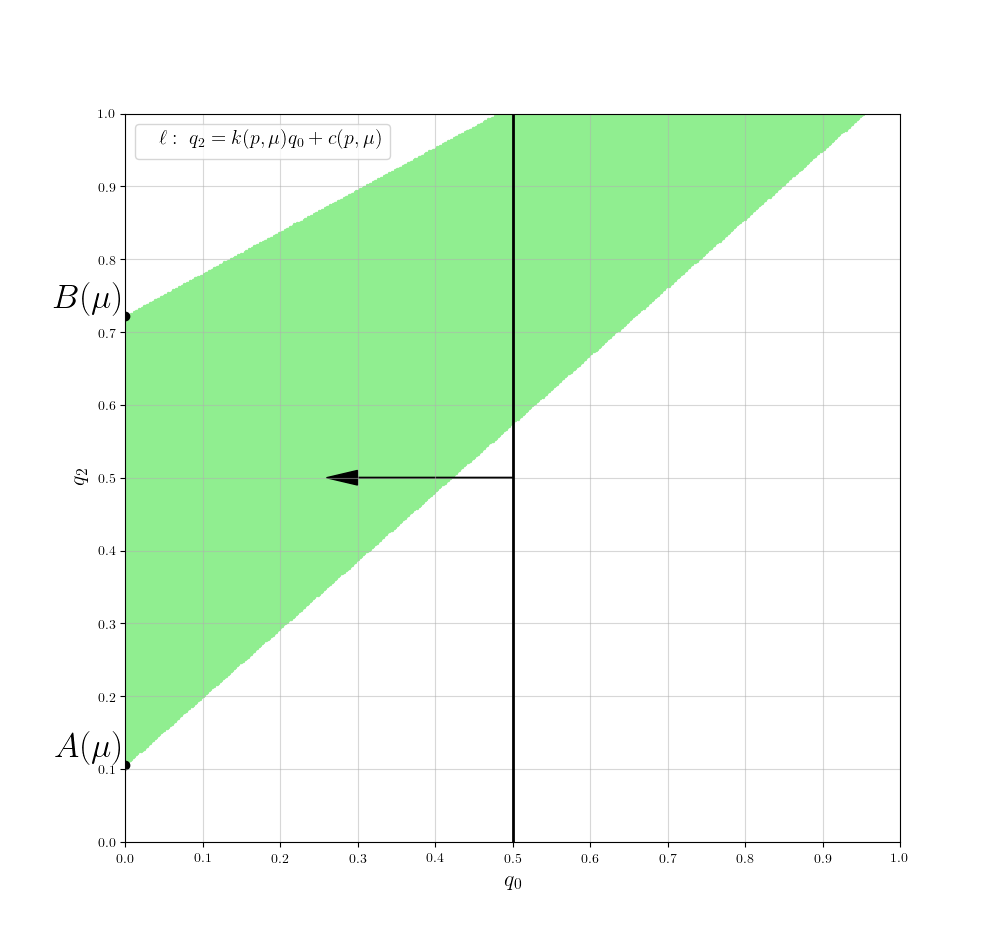
\includegraphics[width=\textwidth]{part_3/graf_3_7_1}
        	\caption{$g_2 = 0 \Rightarrow q^*=[B,A]$}
        	\label{fig:three sin x}
     	\end{subfigure}
     	\begin{subfigure}[b]{0.3 \textwidth}
        	\centering
        	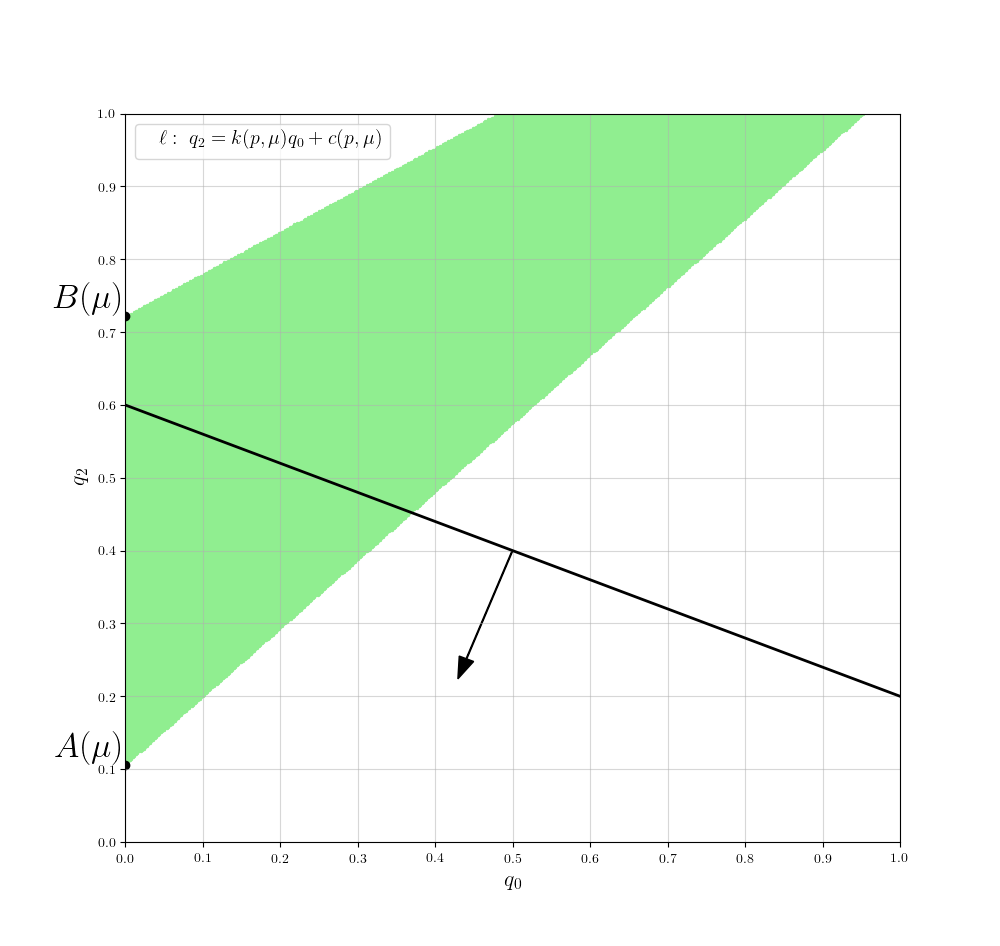
\includegraphics[width=\textwidth]{part_3/graf_3_7_2}
        	\caption{$g_2 < 0 \Rightarrow q^*=A$}
        	\label{fig:three sin x}
     	\end{subfigure}
     	\caption{}
	\end{figure}
	
	\begin{center}
		$\left[
		\begin{gathered}
			g_2 > 0 \Rightarrow q^*=B \\
			g_2 = 0 \Rightarrow q^*=[B,A] \\
			g_2 < 0 \Rightarrow q^*=A
		\end{gathered}
		\right.$	
	\end{center}	
	
	\newpage

	\textbf{(c)} $\frac{1}{3} \leqslant \mu \leqslant \frac{2}{3}$
	
	\begin{figure}[H]
    	\centering
     	\begin{subfigure}[b]{0.3 \textwidth}
        	\centering
        	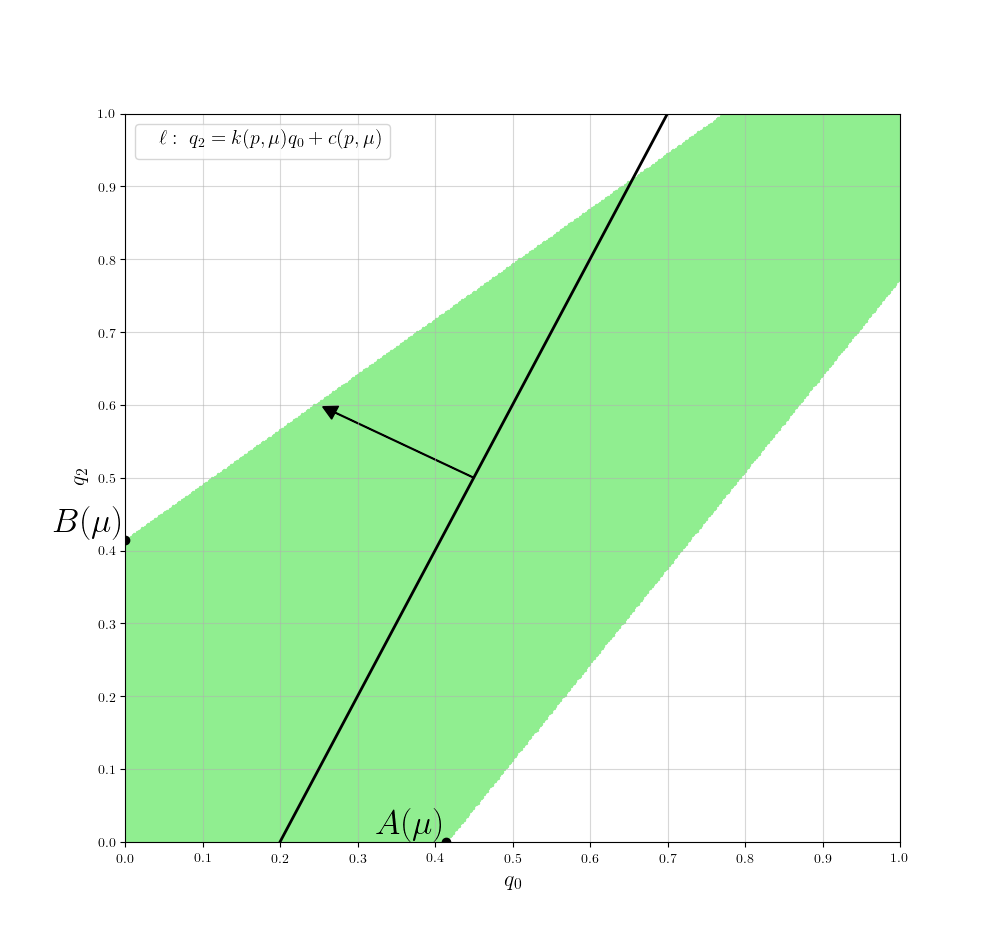
\includegraphics[width=\textwidth]{part_3/graf_3_8_1}
        	\caption{$g_2 > 0 \Rightarrow q^*=B$}
     	\end{subfigure}
     	\begin{subfigure}[b]{0.3 \textwidth}
        	\centering
        	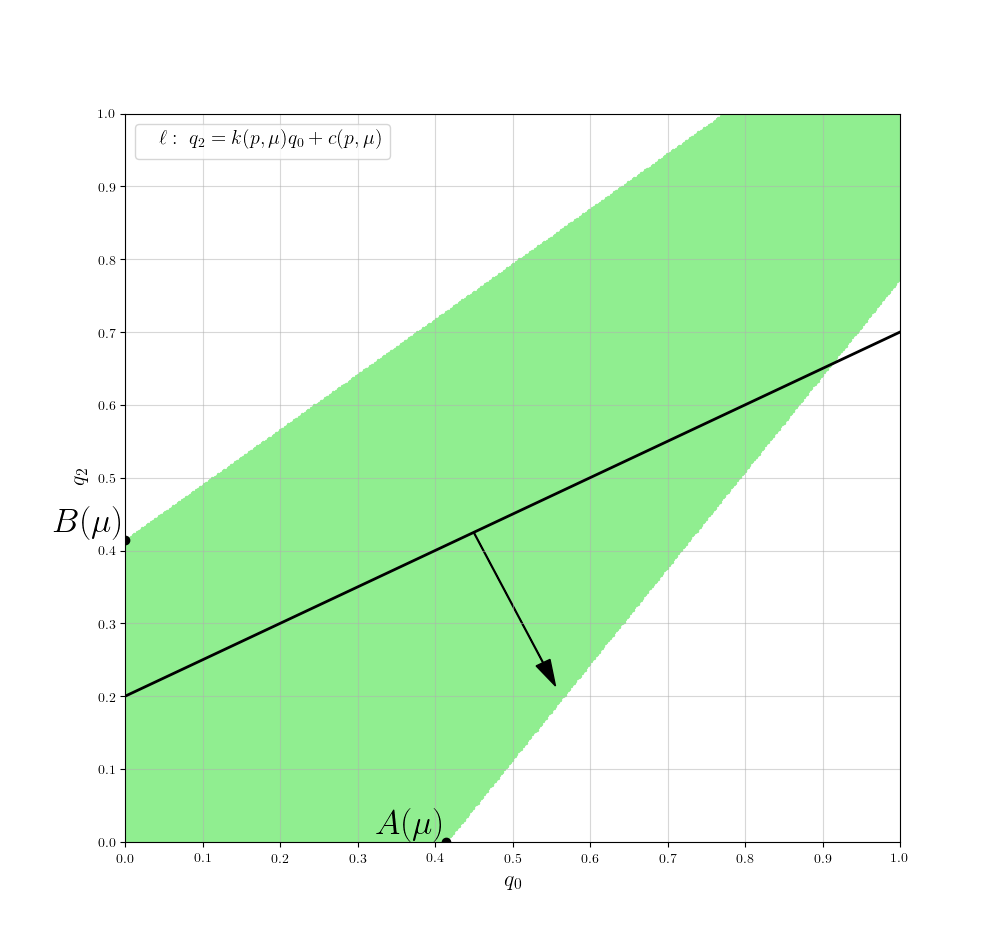
\includegraphics[width=\textwidth]{part_3/graf_3_8_2}
        	\caption{$g_1 > 0 \Rightarrow q^*=A$}
     	\end{subfigure}
     	\begin{subfigure}[b]{0.3 \textwidth}
        	\centering
        	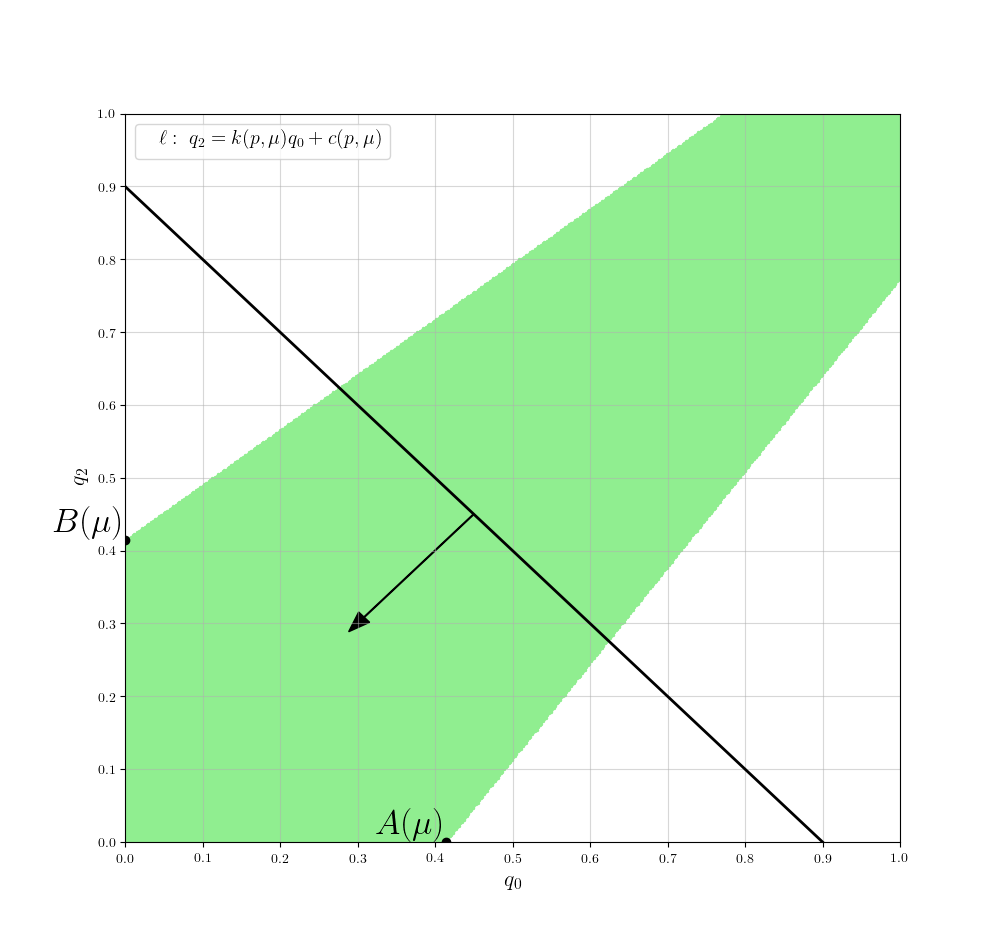
\includegraphics[width=\textwidth]{part_3/graf_3_8_0}
        	\caption{$
        	\begin{cases}			
				g_2 < 0 \\
				g_1 < 0
			\end{cases}	\Rightarrow q^*=(0,0)
			$}
     	\end{subfigure}
    	\centering
     	\begin{subfigure}[b]{0.3 \textwidth}
        	\centering
        	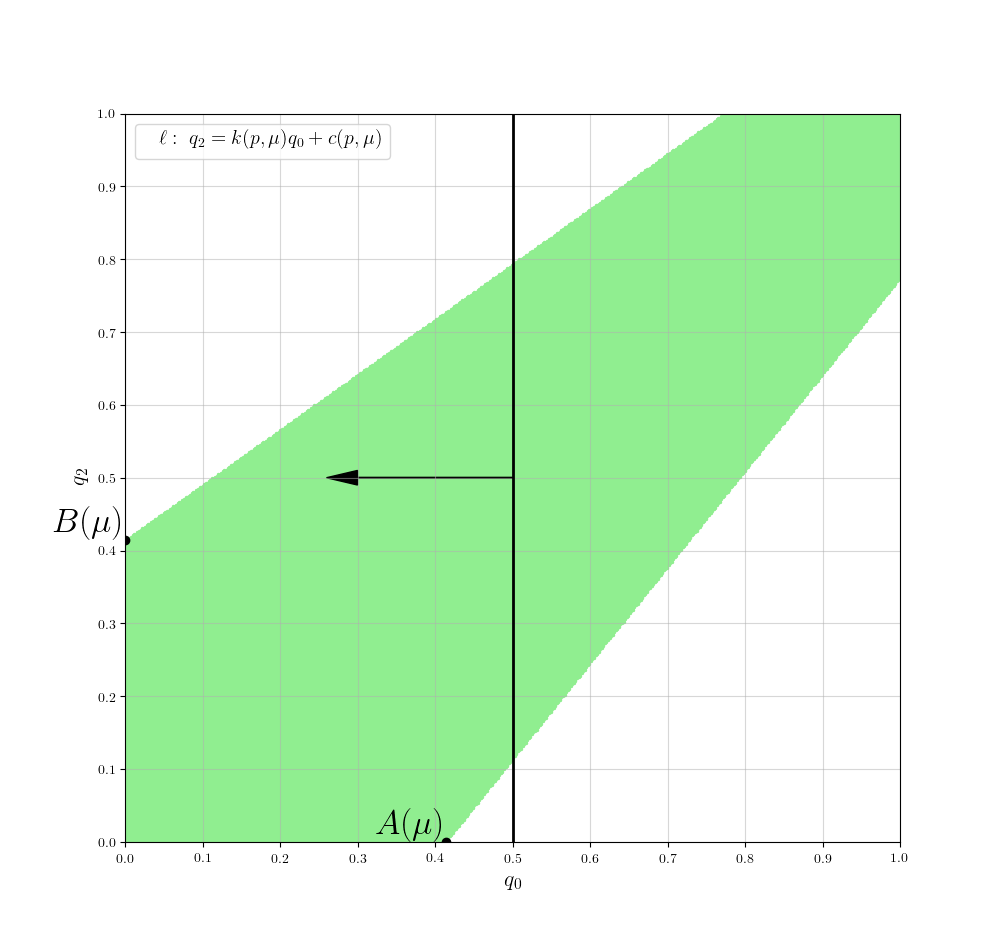
\includegraphics[width=\textwidth]{part_3/graf_3_8_3}
        	\caption{$g_2 = 0 \Rightarrow q^*=[0,B]$}
     	\end{subfigure}
     	\begin{subfigure}[b]{0.3 \textwidth}
        	\centering
        	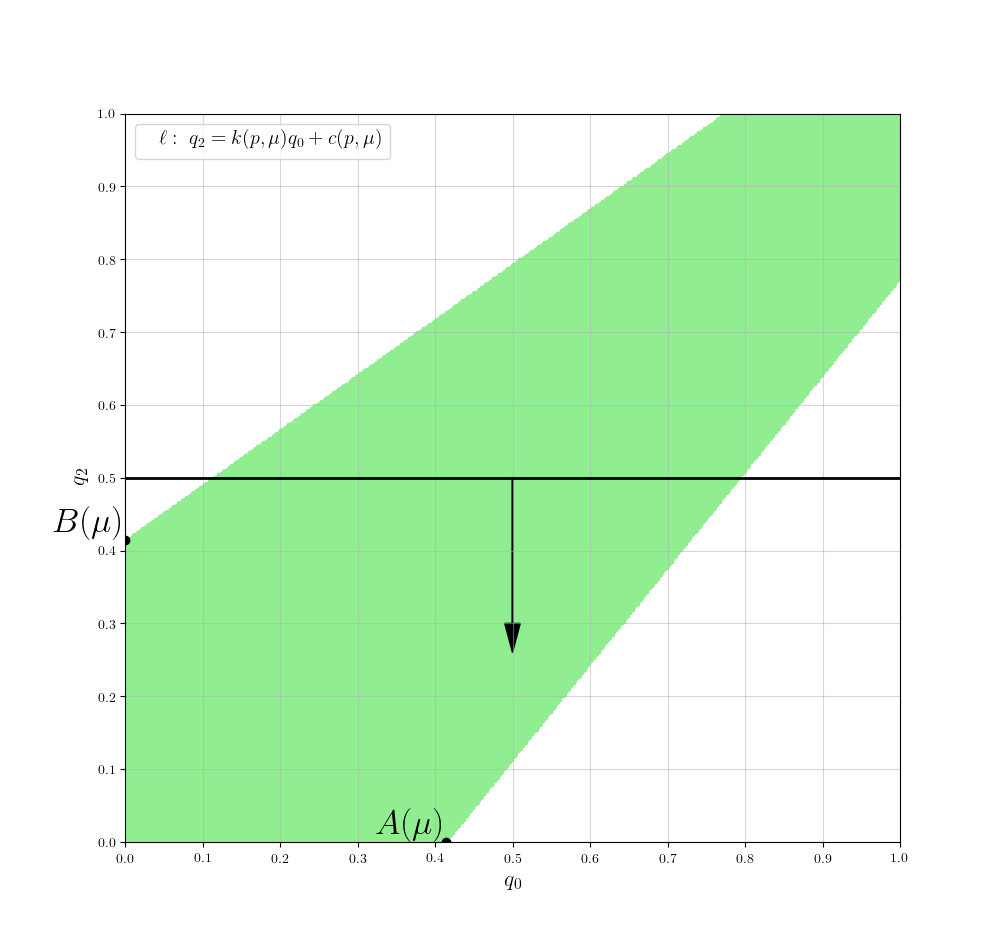
\includegraphics[width=\textwidth]{part_3/graf_3_8_4}
        	\caption{$g_1 = 0 \Rightarrow q^*=[0,A]$}
     	\end{subfigure}
	\end{figure}


	
	\begin{center}
		$\left[
		\begin{gathered}
			g_1 > 0 \Rightarrow q^*=A \\
			g_2 > 0 \Rightarrow q^*=B \\			
			g_1 = 0 \Rightarrow q^*=[0,A] \\
			g_2 = 0 \Rightarrow q^*=[0,B] \\			
			\begin{cases}			
				g_2 < 0 \\
				g_1 < 0
			\end{cases}	\Rightarrow q^*=(0,0)
		\end{gathered}
		\right.$	
	\end{center}

%-------------------------------------------------------------

	Итого получим следующие 

	$C(p,\mu) = \arg \max \limits_{P_{AB}} \overline{G}(p,q,\mu)
	\begin{cases}
	A(\mu), & g_2(p,\mu)<0 \cup \mu \leqslant \frac{1}{3} \cap g_2 < 0 \\
	B(\mu), & g_1(p,\mu)>0 \cup \mu \geqslant \frac{2}{3} \cap g_1 > 0 \\
	(0,0),  & g_1(p,\mu)<0 \cap g_2(p,\mu)<0 \\
	[A(\mu), B(\mu)], 
	& g_1(\mu)=0 \cap \mu < \frac{1}{3} \cup g_1(\mu)=0 \cap \mu > \frac{2}{3} \\
	[0, A(\mu)], & g_2(\mu)=0 \cap \mu \in [\frac{1}{3},\frac{2}{3}] \\
	[0, B(\mu)], & g_1(\mu)=0 \cap \mu \in [\frac{1}{3},\frac{2}{3}] \\
	\end{cases}	
	$	
	
	Но кроме того точки $A(\mu)$ и $B(\mu)$ являются оптимальными 
	$\forall$ $p$ и $\mu$ поскольку	являются таковыми в \textbf{(1)} и \textbf{(2)}.
	Итого в области $P_B$ оптимальной является точка $B(\mu)$,
	в области $P_A$ оптимальной является точка $A(\mu)$,
	и в области $P_{AB}$ оптимальной является точка $C(p, \mu)$.
	Поскольку если $f(x)$ и $g(x)$ непрерывны на множестве $X$, то и 
	$min(f(x), g(x))$ непрерывна на $X$, то максимум достигается в точке
	$C$.
	
	$q^*(p,\mu)= \arg \max \limits_Q \overline{G}(p,q,\mu)
	\begin{cases}
	A(\mu), & g_2(p,\mu)<0 \cup \mu \leqslant \frac{1}{3} \cap g_2 < 0 \\
	B(\mu), & g_1(p,\mu)>0 \cup \mu \geqslant \frac{2}{3} \cap g_1 > 0 \\
	(0,0),  & g_1(p,\mu)<0 \cap g_2(p,\mu)<0 \\
	[A(\mu), B(\mu)], 
	& g_1(\mu)=0 \cap \mu < \frac{1}{3} \cup g_1(\mu)=0 \cap \mu > \frac{2}{3} \\
	[0, A(\mu)], & g_2(\mu)=0 \cap \mu \in [\frac{1}{3},\frac{2}{3}] \\
	[0, B(\mu)], & g_1(\mu)=0 \cap \mu \in [\frac{1}{3},\frac{2}{3}] \\
	(0,1), & \mu = 0 \\
	(1,0), & \mu = 1
	\end{cases}	
	$		
	
	
	%$$g_1=p\mu-(1-p)(1-\mu)  \hspace{10mm}
	%g_1=0 \sim p=\frac{1-\mu}{(\sqrt{2}-2)\mu + 1}$$

	%$$g_2=(1-p)(1-\mu)(\sqrt{2}-1)-p\mu  \hspace{10mm}
	%g_2=0 \sim p=\frac{(1-\mu)(\sqrt{2}-1)}{(\sqrt{2}-2)\mu + (\sqrt{2}-1)}$$
	
	Поскольку в пункте 3.1 мы установили, что 
	
	$$p^*(q,\lambda(q))=\arg \max \limits_{p \in [0,1]}
		\overline{L}(p, q, \lambda(q))=[0,1]
	$$

	Нас интересуют оптимальные пары $(p^0,q^0)$ такие, что 
	$\exists (\lambda, \mu) \in [0,1]^2 $:
	
	$$\begin{cases}
	p^0=p^*(q^0,\lambda) \\
	q^0=q^*(p^0,\mu)
	\end{cases}$$
	
	Введём следующие множества:
	
	$$P_0=[0,1], \; Q_0=[0,1] \times \{0\} \cup \{1\} \times [0,1]$$
	
	Следующие точки являются оптимальными:
	$$(p, q) \in P_0 \times Q_0$$













 % Решения для Студента

	\section{Значение игры}

В предыдущих пунктах были найдены оптимальные стратегии для 
модельной игры с двумя различными значениями параметра дискретизации:
Т=1 и Т=2. Теперь опишем значения игры для оптимальных стратегий при
различных параметрах Т.

\subsection{Значение игры для игрока Студент}

Начнём рассмотрение со случая, когда параметр дискретизации
Т=1. На квадрате $(\mu, \lambda) \in [0, 1]^2$ мы рассмотрели
все точки и для каждой нашли оптимальные пары 
$\big(p^0(\mu, \lambda), q^0(\mu, \lambda)\big)$.
Теперь для всех возможых пар из квадрата
$(\mu, \lambda) \in [0, 1]^2$ в соответсвующих
оптимальных парах найдём значения скаляризованно функции выигрыша 
игрока \textbf{С}:
$$
	\overline G(p^0(\mu, \lambda), q^0(\mu, \lambda), \mu)=
	p \min \Big\{
		\dfrac{q^0}{\mu};
		\dfrac{1-q^0}{2(1-\mu)}
	\Big\} + (1 - p^0) \min \Big\{
		\dfrac{q^0}{2\mu};
		\dfrac{1 - q^0}{1 - \mu}
	\Big\}
$$
Получим следующую систему в зависимости от значений  $\mu$ и $\lambda$:
$$
	\overline G(p^0(\mu, \lambda), q^0(\mu, \lambda), \mu) =
	\begin{cases}
		\dfrac{1}{2}, & 
		\mu = \{0,1\}, \, \lambda \in [0, 1) 
		\\	
		[\frac{1}{2}, 1], & 
		\mu = 0, \, \lambda = 1 \cup 
		\mu = 1, \, \lambda = 0
		\\
		\dfrac{1}{2-\mu}, &	
		\mu \in (0, 1), \, \lambda \in 
		(0, 2\dfrac{1 - \mu}{2 - \mu})
		\\
		\dfrac{1}{1 + \mu}, & 
		\mu \in (0, 1), \, \lambda \in 
		(\dfrac{1 - \mu}{1 + \mu}, 1]
		\\
		\Big[\dfrac{1}{2}, \, \dfrac{1}{2-\mu}\Big], &
		\mu \in (0, 1), \lambda \in 2\dfrac{1 - \mu}{2 - \mu}
		\\ 
		\Big[\dfrac{1}{2}, \, \dfrac{1}{1+\mu}\Big], &
		\mu \in (0,1), \lambda = \dfrac{1-\mu}{1+\mu}
	\end{cases}
$$

Для наглядности и дальнейшего анализа изобразим графически множество
значений выигрыша в оптимальных точках.
Для этого на квадрате $[0, 1]^{2}$ изобразим все значения, которые 
принимает вектор 
$$
	(\mu \overline G(p^0(\mu, \lambda), q^0(\mu, \lambda), \mu)), 
	(1-\mu) \overline G(p^0(\mu, \lambda), q^0(\mu, \lambda), \mu))
$$ 
при всех возможных $(\mu, \lambda) \in [0, 1]^2$. Соответствующий график
изображён на рисунке \ref{fig:EG_1}.

\begin{figure}[H]
	\centering
	\begin{subfigure}[b]{0.47 \textwidth}
		\centering		
		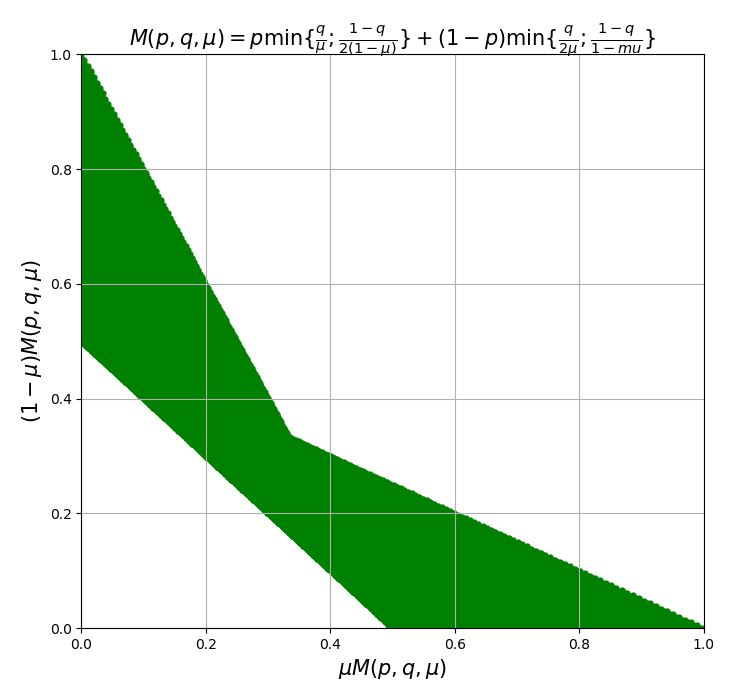
\includegraphics[width=\textwidth]{part_2/graf_4}
		\caption{}
		\label{fig:EG_1}
	\end{subfigure}	
	\begin{subfigure}[b]{0.47 \textwidth}
		\centering		
		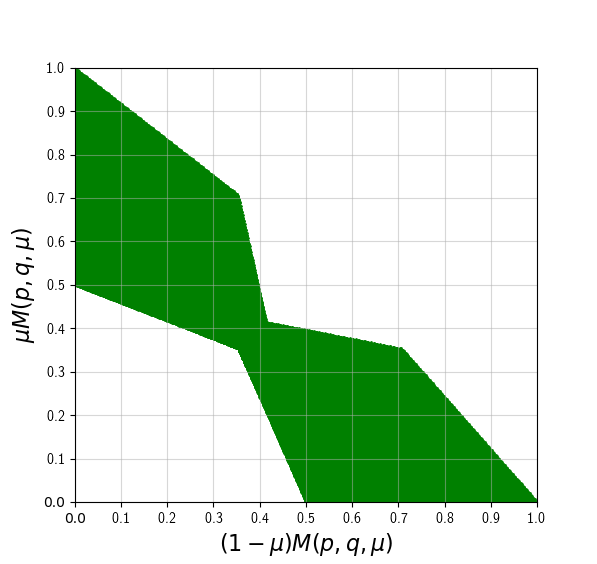
\includegraphics[width=\textwidth]{part_3/Figure_4}
		\caption{}
		\label{fig:EG_2}
	\end{subfigure}
	\caption{}	
\end{figure}

\begin{flushleft}
	Поясним график \ref{fig:EG_1}: \\
	нижняя огибающая в координатах $X,Y$: $y=\dfrac{1}{2}-x$, \\
	верхняя огибающая в координатах $X,Y$: 
	$y=
	\begin{cases}
		1 - 2x, & x \in [0, \frac{1}{3}) \\
		\dfrac{1 - x}{2}, & x \in [\frac{1}{3}, 1]
	\end{cases}
$
\end{flushleft}

Исходя из аналогичных рассуждений получим график для случая Т=2. Он изображён
на рисунке \ref{fig:EG_2}.

 % Значения игры для Преподователя
	\subsection{Значение игры для игрока Преподаватель}

Вернёмся к рассмотрению случая Т=1.
Вычислим матожидание от имеющегося векторного критерия 
\eqref{eq:player_criterion}
, где $x$ и $y$ возьмём как случайные величины с распределениями 
\eqref{eq:probability_1}
и соответсвующими обозначениями велечин $p$ и $q$. В таком случае имеем:

$$
	\mathbb{E}_{xy} [F(x,y)]=
	\Big \langle
		\dfrac{q(1+p)}{2};
		\dfrac{(1-q)(2-p)}{2}
	\Big\rangle
$$

В утверждении 1 мы установили, что любая пара
$(p^0, q^0) \in [0, 1]^{2}$ является оптимальной. 
Рассмотрим это как множество точек на плоскости $X,Y$ зависящие от двух
параметров $(p,q)\in[0,1]^2$

$$
	\begin{cases}
		x = \dfrac{q(1 + p)}{2} \\
		y = \dfrac{(1 - q)(2 - p)}{2}  
	\end{cases}
	\Rightarrow
	\begin{cases}
		q = \dfrac{2x}{1 + p} \\
		y = \dfrac{(1 - \dfrac{2x}{1 + p})(2 - p)}{2}		
	\end{cases}
	\Rightarrow
	\begin{cases}
		q = \dfrac{2x}{1 + p} \\
		y = \dfrac{(1 + p - 2x)(2 - p)}{2(1 + p)}
	\end{cases}
$$

Найдём максимальные значения, которые может принимать $y(x, p)$ при фиксированном $x$:

$$
	\dfrac{\partial y(x, p)}{\partial p}=\frac{3x}{(p+1)^2} - \frac{1}{2} = 0 
	\Rightarrow
	p = \sqrt{6x} - 1
$$

Введём обозначение $p_0 = \sqrt{6x} - 1$. Поскольку область определения 
$p_0 \in [0, 1]$, то $p_0 = 1 \Rightarrow x = \frac{2}{3}$ и 
$p_0 = 0 \Rightarrow x = \frac{1}{6}$
 
$$
	y_{max}(x) = 
	\begin{cases}
		\max \{ y(x, 0), \: y(x, 1), \: y(x, p_0) \}, & 
		x \in \big[ \frac{1}{6}, \frac{2}{3} \big]
		\\
		\max \{ y(x, 0), \: y(x, 1) \}, &
		x \in \big[0, \frac{1}{6} \big] \cap \big[\frac{2}{3}, 1\big]
	\end{cases}
$$
учитывая, что
$
	y(x, 0) = 1 - 2x, \;
	y(x, 1) = \dfrac{1 - x}{2}, \;  	
	y(x, p_0) = \dfrac{(\sqrt{6x} - 2x)(3 - \sqrt{6x})}{2 \sqrt{6x}}
$
получим уравнения верхней и нижней огибающей области на графике ниже.

$
	y_{min}(x) =
	\begin{cases}
		\dfrac{1 - x}{2}, & x \in \big[0, \frac{1}{3} \big] 
		\\
		1 - 2x, & x \in \big( \frac{1}{3}, 1\big]
	\end{cases}
	\qquad
	y_{max}(x) =
	\begin{cases}
		1 - 2x, & x \in \big[0, \frac{1}{6} \big] 
		\\
		\frac{(\sqrt{6x} - 2x)(3 - \sqrt{6x})}{2 \sqrt{6x}}, &
		x \in \big(\frac{1}{6}, \frac{2}{3} \big]
		\\
		\dfrac{1 - x}{2}, & x \in \big(\frac{2}{3}, 1 \big]
	\end{cases}
$

Теперь для всех
оптимальных стратегий т.е. пар $(p^0, q^0) \in [0, 1]^{2}$ изобразим на графике
\ref{fig:EF_1} значения матожидания векторного критерия в этой точке.
Аналогичными рассауждениями для случая Т=2 получаем область на
рисунке \ref{fig:EF_2}:

\begin{figure}[H]
	\centering
	\begin{subfigure}[b]{0.47 \textwidth}
		\centering		
		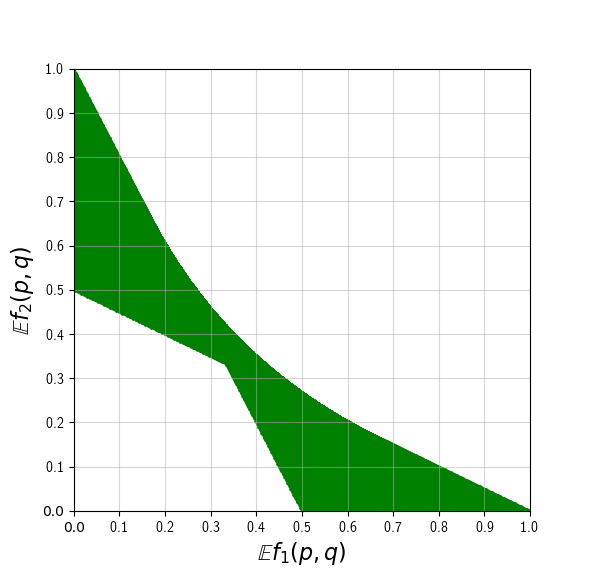
\includegraphics[width=\textwidth]{part_3/Figure_8}
		\caption{}
		\label{fig:EF_1}
	\end{subfigure}	
	\begin{subfigure}[b]{0.47 \textwidth}
		\centering		
		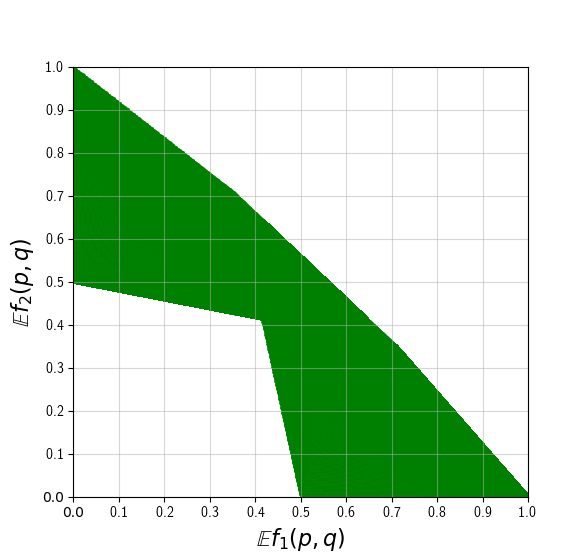
\includegraphics[width=\textwidth]{part_3/Figure_5}
		\caption{}
		\label{fig:EF_2}
	\end{subfigure}
	\caption{}	
\end{figure} % Значения игры для студента

	\section{Заключение}

На примере двухкритериальной игры двух лиц была изучена возможность 
применения линейной свёртки и обратной логической свёртки (кторая 
является модификацией свёртки Гермейера). Рассмотрены два варианта 
дискретизации непрерывной модельной задачи и получены следующие результаты:
\begin{enumerate}
	\item \textbf{Оптимальные стратегии}. В случае Т=1 оптимальные
	стратегии оказались неизирательными, поскольку любая
	допустимая стратения оказалась оптимальной. В случае Т=2
	для игрока \textbf{П} оптимальна любая допустимая сттратегия, а
	для игрока \textbf{С} множество оптимальных стратегий состоит из
	двух отрезков.  
 
	\item \textbf{Множества значений в критериальном пространстве}. 
	Выпуклая оболочка множества значений в критериальном пространстве 
	при оптимальных стратегиях в случае Т=2 содержит в себе это
	множество для Т=1. Более при увеличении степени аппроксимации,
	это множество всё точнее приближается к непрерывному случаю.
	
\end{enumerate}
 % Заключение
	
	% Для соответствия требованиям об оформлении списка литературы
	\bibliographystyle{gost71u} 
	\bibliography{include/bibliogaphy} % Список литературы

\end{document}
